\documentclass[thesis]{template/rrlab}
% !TEX root = thesis.tex

\RRLABtitle{Closed-Loop Control of the Series Elastic Actuator}
\RRLABauthor{Max Erdelmeier}
\RRLABtype{Bachelor Thesis}
\RRLABinception{1. February 2024}
\RRLABsubmission{\today}
\RRLABfirstreviewer{Prof. Dr. Karsten Berns}
\RRLABsupervisor{Oleksandr Sivak}

% needed for \begin{comment}
\usepackage{verbatim}

\begin{document}

\RRLABtitlepage{image?}{\today}

\RRLABsecondpage

\RRLABdeclaration{\today}

\RRLABpreface{Preface}{
    This thesis is the product of many people over many years guiding me on my way.
    So I want to use this opportunity to thank some of them, because I do not do so nearly often enough.
    %Eltern
    %Celina
}

\RRLABabstract{Abstract}{

}

\RRLABcontents

% Here the topic should be introduced, and the structure, goal and scope of the thesis should be defined.
% One should focus on answering the following question: Why is the topic of the Thesis interesting for the (scientific) community?
\chapter{Introduction}
\label{chap:introduction}

\begin{comment}
Rust as new language competitive to C?
Bare-metal still necessary with modern Microprocessors and Real-time Linux?
What if we want to implement something different from linear control?
\end{comment}

\section{Closed Loop Control}
\label{sec:introduction:clc}

Whenever you have a stateful system there are two ways of controlling it.
In Open Loop Control only the should-be signal influences the output value.
In Closed Loop or Feedback Control the output is composed of the should-be value and a feedback signal that measures the actual state of the system.
In many real-world applications Closed Loop Control is used for its ability to quickly reach a new target value, while keeping oscillation and overshoot to a minimum.

For these real-world applications it has been implemented in many different ways,
from mechanical structures like a centrifugal governor to specialized integrated circuits.

In this paper we will implement closed loop control of a brushless DC motor on a Raspberry Pi 4.
This effort is part of the larger goal of building a successor to CARL\cite{CARL} at RRLAB.
There are a variety of different ways the motor controllers could be implemented, the old CARL for example used FPGAs.
We chose to use a Raspberry Pi, because it provides us with some advantages and exciting opportunities.

\section{Advantages of Closed Loop Control on General Purpose Processors}
\label{sec:introduction:gpp}

When compared to the FPGA approach used in CARL Single Board Computers (from now on abbreviated as SBCs) such as a Raspberry Pi are cheaper and easier to program.
This comes at a cost however, typically FPGAs are faster at high speed IO operations, which is an important port of a Closed Loop Controller.
Fortunately the Raspberry Pi 4 has special purpose hardware for SPI and PWM IO which should help us alleviate this disadvantage,
while outperforming the FPGAs in general compute tasks due to the higher clock frequencies.

When compared to ready built PID ICs a Raspberry Pi is more expensive, consumes more power and must be programmed vs only settings a few variables.
But it comes with one major upside for a research project such as ours:
It is not bound to a traditional PID controller. If the need arises to use a different control scheme or compute additional tasks in parallel, the Raspberry Pi can!

In addition, using a Raspberry Pi provides an opportunity to use the Rust programming language and validate some of its claims.

\section{A new programming language for embedded systems?}
\label{sec:introduction:rust}

Systems programming and embedded systems are two closely linked categories.
In both of them the usage of C++ and especially C have dominated that of any other language.
In the last 5-10 years however several new languages have come up,
that claim to be able to replace C and C++ for various parts of the systems programming field.
\begin{itemize}
    \item Go by Google has seen wide adoption in high-performance network related applications, due to its focus on simplicity while maintaining reasonably high performance.\cite{Go}
    \item Zig targets a direct replacement of C for low level systems such as writing operating system kernels or embedded applications. In order to easily integrate into existing C projects the zig compiler can compile both C and Zig files.\cite{Zig}
    \item Carbon directly targets replacing C++ by being able to include C++ files and compiling to the same ABI.\cite{Carbon}
    \item Rust, which was originally developed by Graydon Hoare at Mozilla.\cite{TheRustProgrammingLanguage}
\end{itemize}

The controller implementation in this thesis will be written in Rust,
as that gives us the opportunity to validate some of Rusts claims on its suitability for embedded programs and interoperability with existing SDKs.

To cite the exact quotes we will be looking at in detail:\\
"Interoperability - Integrate Rust into your existing C codebase or leverage an existing SDK to write a Rust application."\\
"Portability - Write a library or driver once, and use it with a variety of systems, ranging from very small microcontrollers to powerful SBCs."\\
\cite{RustEmbeddedSite}

In order to do that we will implement the controller twice.
Once running bare-metal while using the Circle library for interacting with the hardware,
and second while running on a standard linux kernel on the Raspberry Pi.
This allows us to compare the effort of writing an embedded application in Rust to the effort
when writing the same application on top of a general purpose operating system.
The Circle library is a C/C++ SDK for all Raspberry Pis which will serve as our test bed for exploring Rust's C interoperability.

Since we will be taking a detailed look at some of Rusts features let us provide some general information on the language.

Rust was designed to be a similarly performant alternative to C and C++ while eliminating some of their most common pitfalls:\\
\begin{itemize}
    \item buffer overflows
    \item out of bounds read
    \item race conditions
    \item reading uninitialized memory
    \item dereferencing null pointers
\end{itemize}

It does this through a combination of approaches where the most important ones are RAII through an ownership system and a lifetimes for references instead of pointers.
We will cover these in more detail in the background (\ref{background}) chapter.

\chapter{Background}
\label{chap:background}

% This question should answer the question: How did others try to solve the problem, and what did they miss?
% So, why is the problem not yet solved? In short, this should define the research gap of your work.
% For this, state-of-the-Art approaches should be described.
\chapter{Related Work}
\label{chap:related_work}

The idea of using SBCs for embedded systems tasks is not new.
The advantages of short test cycles, flexible implementations and a for the programmers familiar environment make general purpose processors seem very enticing for embedded systems.
This in combination with the spread of Raspberry Pis has led to similar research to our paper.

\section{Rasbperry Pi Research}

In \textit{Raspberry Pi performance analysis in real-time applications with the RT-Preempt patch} \cite{Rasp3}
the timing behavior of a Raspberry Pi 3 with the PREEMPT-RT patch is investigated.
This includes a test polling a GPIO input,
a test for reaction times to hard- and software interrupts,
and a test running a ping-pong loop between two Rasbperry Pis with a one millisecond delay.

Although these tests are not directly comparable to our tests, as we mainly output things, while they tested input latencies, there is still very valuable information for us in this paper.
When we look at the test results for the timed loop test in Figure \ref{fig:rasp3}, we can see that they observed maximum latencies of three to eight times the minimum latencies.
If this translates into the worst-case latencies for our testing later, it would render the Linux version unsuitable for our goal.

\begin{figure}
  \begin{center}
    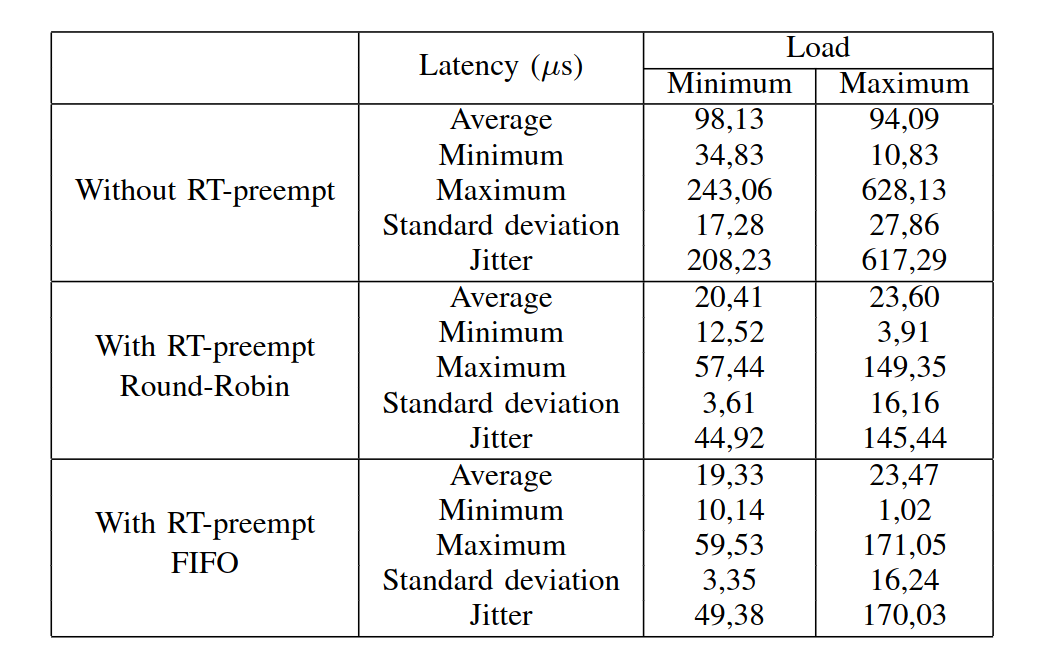
\includegraphics[width=.8\textwidth]{assets/Rasp3.png}
    \caption{Timed loop test results from \cite{Rasp3}}
    \label{fig:rasp3}
  \end{center}
\end{figure}

Almost identical research has been done on the Raspberry Pi 3 in \textit{Real-Time Performance and Response Latency Measurements of Linux Kernels on Single-Board Computers} \cite{computers10050064}.
This paper also used the ping-pong loop between two Raspberry Pis for the reaction time measurement.
There are some small differences to the former paper:
\begin{enumerate}
  \item For comparison the paper includes the Beagle Bone Black SBC
  \item The kernels tested are the far older 4.14 and 4.19 kernels
  \item The paper also considers multiple Linux distributions (Ubuntu, Arch Linux, and Debian), which can affects the tools and flags to compile the kernel.
\end{enumerate}
Interesting here are the results in comparison with the former paper, for the Debian version, which had the newest kernel, the minimum response time was 40$\mu$s and the maximum 90 $\mu$s.
One possible explanation for the much higher latencies than in the former paper could be the comparatively old kernel version.

Similarly, \textit{A Performance Evaluation of Embedded Multi-core Mixed-criticality System Based on PREEMPT RT Linux} \cite{Rasp4},
tests latency and throughput characteristics with PREEMPT-RT on the Raspberry Pi 4.
Although this is the same hardware as we use, there are some important differences:\\
They propose an approach that divides real-time and best-effort tasks by running the best-effort tasks on a virtualized unmodified Linux kernel.\\
They measure task wake-up times using cyclitest, a tool developed together with PREEMPT-RT, while we test for our specific use case and compare to a bare-metal version.\\

During the writing of this thesis the new Raspberry Pi 5 was released, with a faster processor and more IO capabilities.
Does this mean that our research is already outdated?\\
Not necessarily, similar to the Raspberry Pi 4, the Raspberry Pi 5 suffers from supply bottlenecks,
as demand outpaces the production capacity of the Raspberry Pi foundation, making Raspberry Pi 4s cheaper and more readily available.
Additionally many improvements of the Raspberry Pi 5 are more benefitial for server style tasks as opposed to embedded systems:
\begin{itemize}
  \item The additional IO capabilities of the Pi 5 are just more and faster PCIe lanes, which has very little relevance for embedded systems and especially our use case.
  \item The addition of a real-time clock to have persistent time across reboots is of little importance for our use case.
  \item The faster processor may only benefit our system marginally, as the IO times on the Pi 4 are already significantly slower than the computations.
\end{itemize}

Still, there will be some benefits to the Pi 5 and there is already some preliminary research on its real-time capabilities.
\textit{A Preliminary Assessment of the real-time capabilities of Real-Time Linux on Raspberry Pi 5} \cite{Rasp5} examines the real-time capabilities of the Raspberry Pi 5 using cyclitest,
similar to \textit{A Performance Evaluation of Embedded Multi-core Mixed-criticality System Based on PREEMPT RT Linux} \cite{Rasp4}.
In Figure \ref{fig:rasp4} and \ref{fig:rasp5}, we compare the results of the two papers.
This comparison is interesting because according to these results, the Pi 4 is better at real-time operations at the moment.
This may be because Linux is not yet fully optimized for the architecture of the new bcm2712 processor.

\begin{figure}
  \begin{center}
    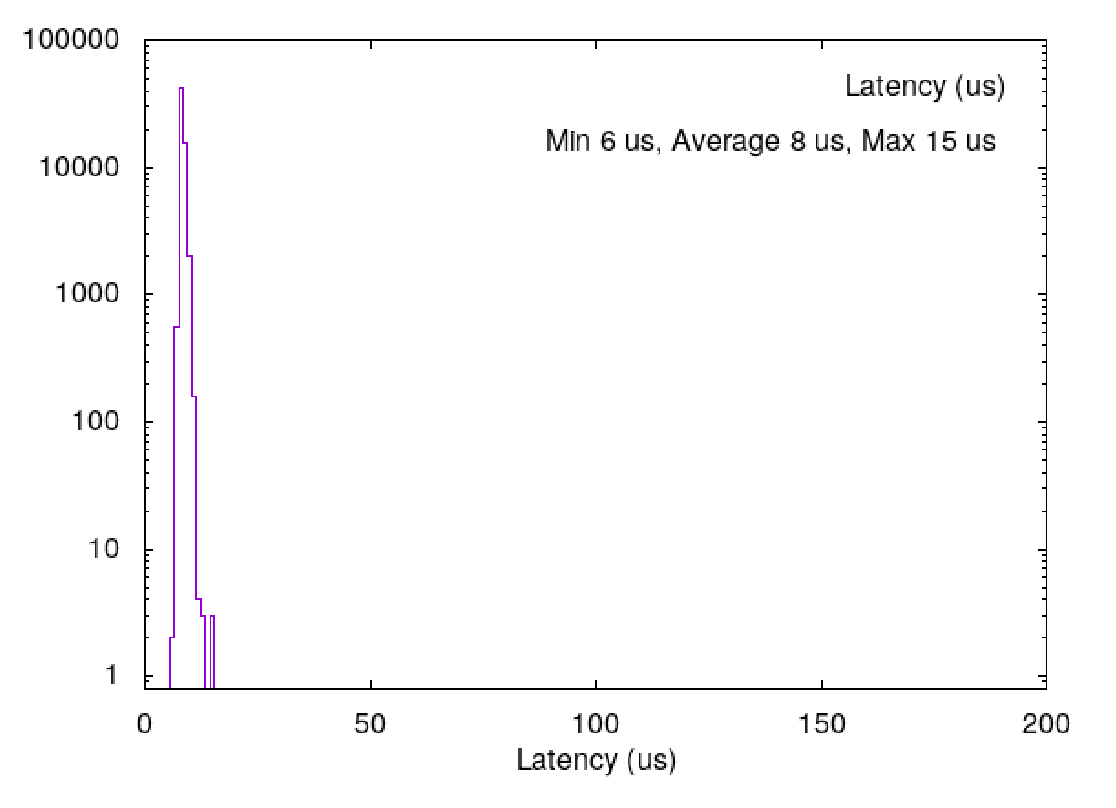
\includegraphics[width=.8\textwidth]{assets/Rasp4.png}
    \caption{Kernel scheduling latency on the Raspberry Pi 4 measured with cyclitest \cite{Rasp4}}
    \label{fig:rasp4}
  \end{center}
\end{figure}

\begin{figure}
  \begin{center}
    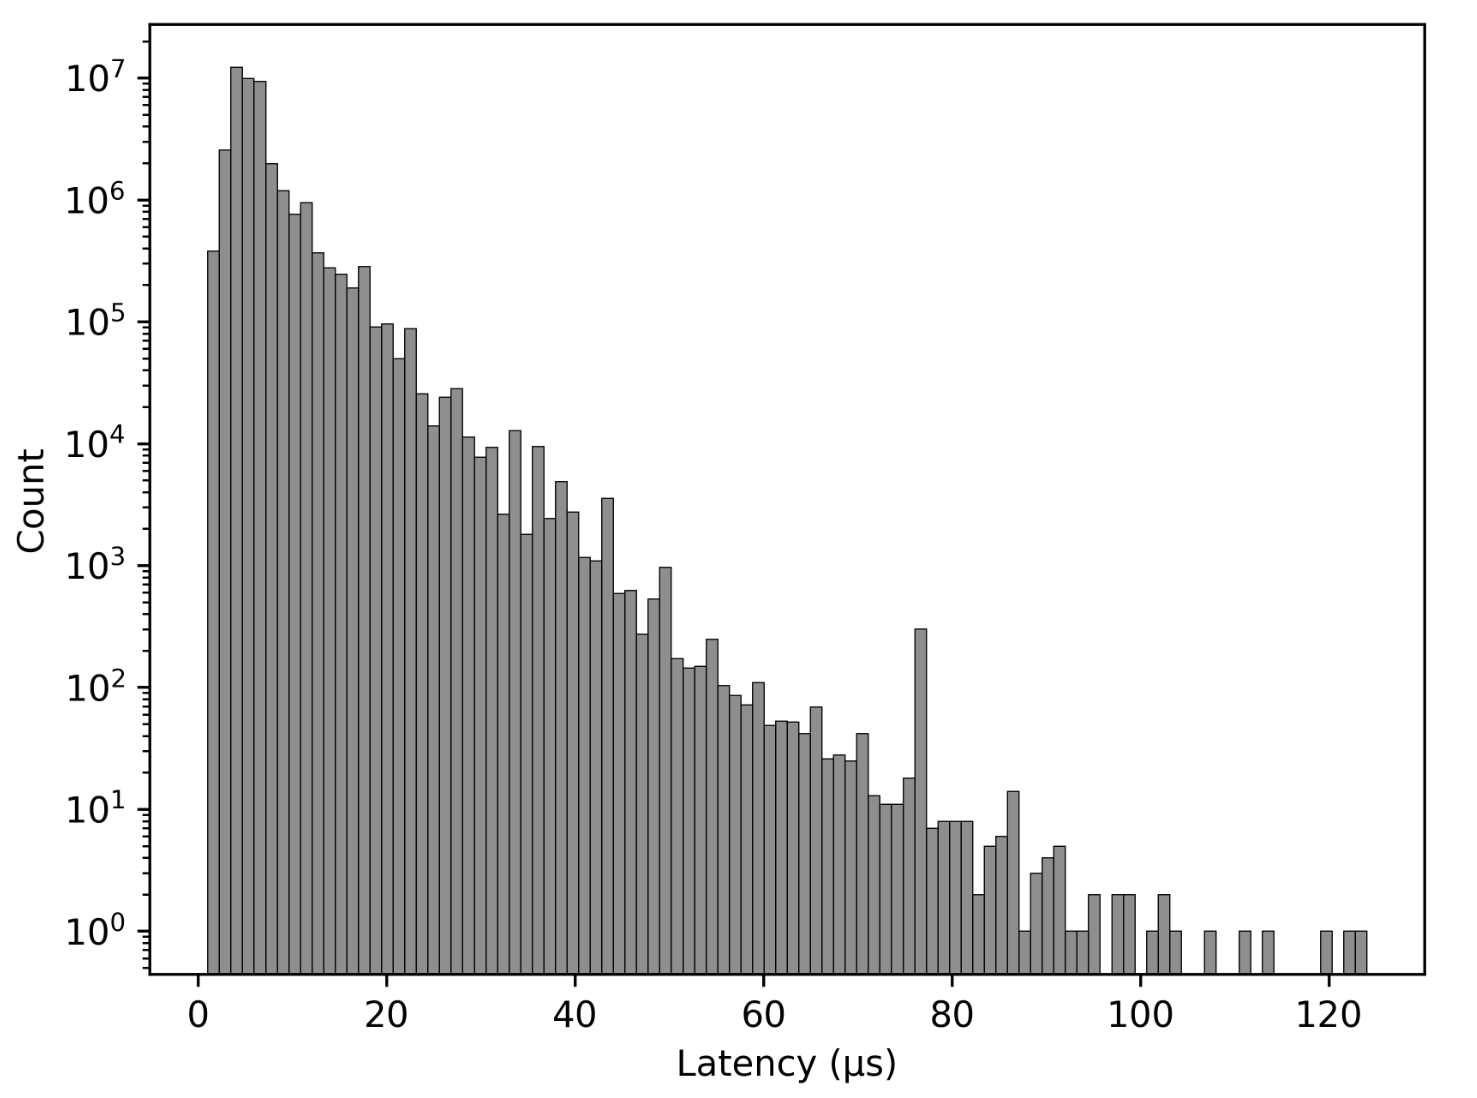
\includegraphics[width=.8\textwidth]{assets/Rasp5.png}
    \caption{Kernel scheduling latency on the Raspberry Pi 5 measured with cyclitest \cite{Rasp5}}
    \label{fig:rasp5}
  \end{center}
\end{figure}

\section{Rust for embedded systems}

Rust's usage for embedded systems is a very active research area.
The research can be roughly split into two categories:
\begin{enumerate}
  \item Evaluating new approaches that are made possible by Rust's modern features, like the borrow checker and zero sized types.
  \item Evaluating how Rust solves old problems with already known solutions.
\end{enumerate}

In the first category, research into embedded operating systems is a very common target.
A very prominent example of this is the Tock RTOS \cite{tock}, a Rust-written OS kernel with a strong focus on security.
For this RTOS alone, there are already papers investigating the general architecture \cite{tock2}, the limitations \cite{theft}, possible solutions \cite{tock3}, and the security model \cite{tock4}.

But since our research clearly falls into the second category, we will focus on that.
For an up-to-date overview of the general state of Rust, \textit{Rust for Embedded Systems: Current State, Challenges and Open Problems} \cite{sharma2023rustembeddedsystemscurrent} is a recent paper that focuses on a general overview.
The important part for us here is their second research question:\\
Interoperability of RUST. How well can RUST interoperate with existing C codebases and what are its challenges?

Because this is closely related to our own Rust research, this opens up a few questions.
How did they investigate the question? What did they find, and how does it relate to our research?

For this research, they developed a simple Rust application on top of FreeRTOS,
a common RTOS written in C, and the same application in C built on top of a Rust port of FreeRTOS.
We will later only look at the direction Rust on top of C.
The results of their research are two findings:
\begin{quotation}
  Significant development effort is required to engineer a C embedded application on top of RUST RTOSes.
\end{quotation}
\begin{quotation}
  It is easy to convert a self-contained, embedded system component of C RTOS into RUST.
\end{quotation}

There is one big difference in our research, however, that could lead to a different conclusion than they have;
Our project will be built upon the Circle library, which is a C++ library, that provides a mostly C-style API,
but has some functions that make use of inheritance.

% This is the first main part of the thesis.
% Here the approach you and your supervisor decided on should be explained.
% Usually, first on a higher level and then in detail including implementation details.
% So the question that is answered is: How do you try to solve the problem at hand?

\chapter{Concept and Implementation}
\label{chap:concept_and_implementation}

In this chapter, we will first consider the general control flow of our application, both for the bare-metal and OS based versions.
For the Linux version specifically, we will then compare multiple approaches to optimize the OS both in terms of average performance as well as worst-case latencies.
These different versions will be compared later to the bare metal version in the \nameref{chap:experiments} chapter.
The bare-metal version demands a more detailed look, as it is the focus of this thesis.
For the bare-metal version, we will first look at the bootup process on the Raspberry Pi and how to produce a Rust binary that successfully boots.
From that we will continue with how the bindings to Circle were created as well as how and why an abstraction on top of it was written to make the underlying C code adhere to Rust's safety guarantees.

\section{The Control Loop}
\label{sec:concept_and_implementation:control_flow}

The general control flow follows the principle of a superloop.
On startup we initialize the communication hardware and from there on it is just a fetch, compute, update loop.
In the fetch step, we get the current position of the actuator, the control value and the time since the last cycle.
The position is fetched through SPI from the IC-MU and the duration since the last cycle from a CPU timer.
For increased reproducibility, we will mock an external control value input by replacing it with a fixed signal based on timers on the Raspberry Pi.
In the compute step, we apply those values to our PID-controller formula to get the new output value.
Finally, in the update step, we update the duty cycle of the output PWM signal based on the just computed output value.

\section{Linux based version}
\label{sec:concept_and_implementation:linux}

Interacting with the SPI and PWM hardware on Linux works through the spidev character device in /dev/spidev0.0 and the pwm interface in /sys/class/pwm.
For Rust there exists a library called rppal that provides a simple interface for interacting with these.
Because of this, it will be used for the Linux versions.

\subsection{Approaches to minimize jitter}
\label{sec:concept_and_implementation:linux:approaches}

In order to give the Linux version the best chance to compete with the bare-metal version, we try two optimization approaches.
First, we tell the Linux scheduler to reserve an entire core for our program, so that it is never moved between cores and never interrupted by core local interrupts.
By this we aim to improve the worst-case iteration times without changing the average case.
In an attempt to go even further we will also try a Linux kernel with the PREEMPT\_RT patchset,
which replaces the scheduler by a real-time capable one and makes every section of the kernel preemptible.
The idea behind this is that even the parts of our program that run in kernel space,
by making syscalls to the spi and pwm kernel drivers, run at a higher priority than other kernel tasks.
To verify if our approaches made any significant difference, we will also be running an unmodified stock kernel with our program at default priority.

\subsection{Setup with rppal}
\label{sec:concept_and_implementation:linux:rppal}

Setting up Spi and PWM through rppal isn't very complex,
but it comes with a few small caveats that are noteworthy
and is a good primer on how linking to external code works in Rust which will be useful when we turn to the bare-metal version.

Rust projects are built using the Cargo build system. This allows us to add rppal into the compilation process by editing our projects Cargo.toml file.

\lstinputlisting[]{code/os-based/Cargo.toml}

Without going into too much detail, the Cargo.toml first specifies some metadata about our project, such as name, version, and the edition.
The edition is a language standard specifier similar to C99 vs C11 and 2021 is the latest at the time of writing.
Rust editions typically get released every three years and are backwards compatible.
Afterwards, the dependencies are specified with versions and optionally feature flags and where to pull them from.
By default, this pulls the rppal source code from crates.io and builds it together with our program and links the two afterwards.
Alternatively, we could have specified a link or path to a custom version of rppal if that were needed.
Then, setting up the devices is done by including the relevant types and creating instances of them.

\lstinputlisting[language=Rust,style=colouredRust,linerange={5-9,36-42}]{code/os-based/src/lib.rs}

On a stock Raspberry Pi 4 with Raspberry Pi OS this would still fail, because by default the spi and pwm device tree overlays are not enabled.
In order to enable them, we need to set dtparam=spi=on in /boot/firmware/config.txt for spi and dtoverlay=pwm for pwm.

\subsection{Getting the current position}

In \nameref{sec:background:hardware:spi} and \nameref{sec:background:hardware:ic-mu} we have already seen how SPI and the position encoder that we use work.
This leaves us with the question of how to transmit the actual position data.
The position transmission is initiated by the SPI master by sending the SDAD\_TRANSMISSION opcode.
The IC-MU chip responds by echoing the opcode and appending the position.
The format and length of the position are dependent on several configuration values on the IC-MU, but for our purposes the default configuration is appropriate.
In the default configuration, this is 19 bits of actual position data with five zeros added as padding.
In Rust, the transmission looks like this:

\lstinputlisting[language=Rust,style=colouredRust,linerange={44-52}]{code/os-based/src/lib.rs}

Here we transmit by writing in the same buffer that we are reading from for sending, which means that we need four bytes of space, one for the opcode and 3 for the data.
To make converting to an integer easier, we add a fifth byte, so we can just interpret the last 32 bits of the buffer as our position.
Because the IC-MU sends in big endian, we use u32::from\_be\_bytes() for the conversion.

\subsection{Providing a PID controller}

While the aim of this thesis is to enable flexible implementation of different control schemes, implementing these is not in our scope.
For now, we will implement a simple PID controller that stays the same between the Linux and bare-metal versions.

For this we decided on the pid-ctrl library to be used, as it is easy to use, works on bare-metal, and supports differing time deltas.

The process of including it is analogous to rppal.
In fact in the \nameref{sec:concept_and_implementation:linux:rppal} chapter,
we already included it in our build process and created an instance of the Pid type.
So, all that is to do is to use it inside our main loop.

\lstinputlisting[language=Rust,style=colouredRust,linerange={10-34}]{code/os-based/src/lib.rs}

\section{Bare-Metal}
\label{sec:concept_and_implementation:bare_metal}

Bare metal programming is traditionally something reserved for microcontrollers or OS kernels.
While the Raspberry Pi 4 is not a microcontroller but a fully fledged PC capable of running desktop class operating systems,
its simple boot process and access to low level IO such as $I^2C$, SPI and GPIO pins capable of analog input and output still allow it to be used, as if it were a microcontroller.

\subsection{HAL vs Circle}
\label{sec:concept_and_implementation:bare-metal:hal}

As we have seen in \nameref{sec:background:rust:embedded} the traditional way to program for a microcontroller in Rust
is to create a library for it that implements all the traits from the embedded-hal crate and a second library for the bootup process.
Doing that from scratch is a significant task that would exceed the scope of a bachelor thesis by quite a bit.
But in order to enable a better evaluation of Rust's suitability for embedded systems, we will demonstrate how such an implementation would look for the Gpio pins in \nameref{sec:concept_and_implementation:hal}.
For the actually functional bare-metal program, we will be using a different route.
The Circle library is a C++ framework that provides bare-metal access to pretty much all of the Rpi's available hardware.
That means not only Gpio, Spi, and I2c, but also the more complex subsystems, such as PCIe, USB, display outputs, and ethernet.
So we are going to use this library through Rust's Foreign Functions Interface (FFI from now on).

\subsection{Cross compiling for bare-metal aarch64}
\label{sec:concept_and_implementation:bare-metal:cross}

On Linux there are two main ways to obtain a Rust compiler.
Through your distributions package manager or through rustup,
a tool for managing if necessary multiple versions of rustc, as well as any connected tooling.
For cross compilers, the first option is nearly nonexistent, so we need to use rustup.
Rustup is easily installed on Linux by running the following command.
\begin{verbatim}
curl --proto '=https' --tlsv1.2 -sSf https://sh.rustup.rs | sh
\end{verbatim}
To be able to cross compile to aarch64-unknown-none we run
\begin{verbatim}
rustup target add aarch64-unknown-none
\end{verbatim}
For most targets the rustup target add command does two things.
First, it downloads the compiler backend for the new target architecture.
Second, it downloads a precompiled version of the rust standard library for the new target if available.
Since we are adding a bare-metal target, there is no complete standard library, but Rust's standard library is split into three parts, of which we can use two.
The lowest and most constraint part is the core library.
It contains primitive types and operations on them.
Because this part is built purely on llvm primitives it is available for every target and does not need to be compiled as it lives inside the compiler.
The second part available to bare-metal systems is the alloc library, which adds types, operations, and traits that depend on the existence of a memory allocator.
If we want to use this part, we need to provide a memory allocator.
Fortunately for us, Circle provides a malloc and free implementation, which we can use as our allocator.
The third part of the standard library is called std and contains all types that rely on syscalls to the underlying operationg system.
This means networking, file system access, and timing.

If we are only cross-compiling rust code this would already be enough.
But since we also want to compile Circle and then link the final binaries together, we need a C cross compiler as well as a linker.
Arm provides precompiled toolchains for C, so we will use the latest one provided by them at the time of writing.
%https://developer.arm.com/downloads/-/arm-gnu-toolchain-downloads

There is one final thing to do, when linking to external binaries Rust uses \$\{target\}-gcc as the linker, so in our case aarch64-unknown-none-gcc.
To use aarch64-none-elf-ld instead which we got from Arm in our project directory we add a .cargo/config.toml file with the following content:
\begin{lstlisting}
[target.aarch64-unknown-none]
linker = "aarch64-none-elf-ld"

[build]
target = "aarch64-unknown-none"
\end{lstlisting}
The linker line sets the linker to the correct binary and the target lines changes the default target when using cargo.

\subsection{Bootup process of the Raspberry Pi 4}
\label{sec:concept_and_implementation:bare-metal:boot}

The first part of creating a bare metal controller is creating a binary that even boots on the Raspberry Pi.
\begin{enumerate}
    \item The on-chip first stage bootloader is loaded from address 0x60000000
    \item It checks if a recovery.bin is present on the first FAT32 partition of the SD-card. If it is found, it is flashed to the onboard EEPROM chip and the Rpi is rebooted.
    \item Else it loads the second stage bootloader and its configuration from the EEPROM
    \item The second stage bootloader loads the third stage bootloader either from the SD-card, a USB storage device or the network, depending on the configuration.
          The third stage bootloader is split into the binary start4.elf, the relocation table fixup4.dat, and config.txt for the configuration.
    \item The third stage bootloader loads the kernel image and jumps to address 0x80000. By default, this is kernel8.img, but the kernel file name can be set in config.txt.
    \item In some cases, this kernel.img may be another bootloader such as u-boot, which could then load grub.
          This additional boot part is used in many linux distributions that support uefi boot on aarch64 and not the Raspberry Pi specific chain.
\end{enumerate}

To produce a bootable rust binary we start from a clean project folder generated with cargo new.
This clean project contains a Cargo.toml for the build system configuration and a src/main.rs with the actual code.

First, we will add a .cargo/config.toml similar to what we saw in \nameref{sec:concept_and_implementation:bare-metal:cross}.
\begin{lstlisting}
[target.aarch64-unknown-none]
linker = "aarch64-none-elf-ld"
rustflags = ["-C", "link-arg=Tlink.ld"]
    
[build]
target = "aarch64-unknown-none"
\end{lstlisting}
The added rustflags line allows us to control which logical addressess code is placed at in the linking step.
To control this, we create link.ld:
\begin{lstlisting}
SECTIONS
{
    . = 0x80000;
    .text :
    {
        *(.text._start)
        *(.text*)
    }
}
\end{lstlisting}
The .text section of a binary is where the actual instructions lie as opposed to .data and .bss.
What we are doing here is keeping all the segments in .text, placing .text.\_start at the beginning of .text and letting .text begin at 0x80000.
As we already discussed, 0x80000 is the address to which the Raspberry Pi jumps after loading the kernel.
Now for the actual Rust code. Since there is no standard library on bare metal, we need to tell Rust not to link to the standard library.
This is done by prepending \#![no\_std] to main.rs.
The second thing to prepend is \#![no\_main] because otherwise Rust expects a main function that can be called with the runtime setup required for command-line arguments.
On bare-metal we neither have command-line arguments nor a runtime.
One thing that the standard library provided for us was a panic\_handler implementation.
As the name suggests, the panic handler controls panic exceptions.
On an operating system that typically includes logging the error message to stderr, but for bare-metal Rust expects us to provide an implementation.
That leaves one final task, writing the function that will actually be run and ensuring that it is linked to the .text.\_start section.
\begin{lstlisting}[language=Rust,style=colouredRust]
#![no_std]
#![no_main]

use core::panic::PanicInfo;

#[panic_handler]
fn panic(_: &PanicInfo) -> ! {
    loop {}
}

#[no_mangle]
#[link_section = ".text._start"]
pub extern "C" fn _start() -> ! {
	loop {}
}
\end{lstlisting}

The \#[no\_mangle] attribute before the start function tells the Rust compiler not to mangle the function name, which it would do by default.
The \#[link\_section] attribute ensures that our start function is linked to the section we forced in the linker script to be included at address 0x80000.
The pub attribute makes the function visible to the linker instead of only to the compiler.
The extern C attribute tells the compiler to adhere to the C ABI (Application Binary Interface) for the start function.
This is necessary because the Rust ABI is unstable and may be more complicated than jumping to the start address.

At this point, we can obtain a binary by running cargo build.
But this binary would be an elf executable that cannot be executed without a program loader.
ELF in this context stands for executable-linkable-format and is the file format that linux expects for executable binaries,
with a header that contains all the relevant information for the dynamic linker.
The bootloader, however, just copies the kernel image to RAM and sets the instruction pointer to 0x80000.
This means that we have to rip out the code from our elf binary and create a flat binary without an elf header.
The program that does this is called objcopy and is a standard part of the gnu toolchain.
This means that we already have the correct version aarch64-none-elf-objcopy available from installing the C cross-compiler.

\begin{verbatim}
cargo build --release
aarch64-none-elf-objcopy -O binary \
    target/aarch64-unknown-none/release/<project-name> \
    kernel8.img
\end{verbatim}

When building a Rust only bare-metal project, there is an easier way to obtain objcopy than to install the complete Gnu toolchain.
\begin{verbatim}
rustup component add llvm-tools
cargo install cargo-binutils
\end{verbatim}
Which allows to build and extract the binary in one command with any target available that was added through rustup.
\begin{verbatim}
cargo objcopy --release -- -O binary kernel8.img
\end{verbatim}

\subsection{Compiling Circle and linking it to Rust}
\label{sec:concept_and_implementation:bare-metal:ffi}

Many languages provide a way to link to C ABI functions; examples for this are C++ with its extern C, Haskell with its FFI module, as well as Python.
The reasons for this are very simple; for one, the C ABI for each target platform is stable and allows thus to be used as a common language to bridge other languages.
Second, C is still a widely used language with many useful libraries in any field of programming, which can then be used by languages with a C interface.

As Rust is a systems programming language, the prevalence of C libraries in areas interesting to Rust is even greater.
In its most basic form, the Rust FFI system works through declaring functions as extern C, when calling Rust functions from C
and declaring extern C functions in Rust without a definition, when calling C code from Rust.

\begin{lstlisting}[language=Rust,style=colouredRust]
use std::ffi::c_int;

extern "C" {
    fn c_function(number1: c_int) -> c_int;
}

#[no_mangle]
pub extern "C" fn rust_function(number2: c_int) -> c_int {
    number2
}

fn calling_c_from_rust() {
    let _ = unsafe { c_function(42) };
}
\end{lstlisting}

\begin{lstlisting}[language=C]
int rust_function(int number2);

int c_function(int number1) {
    return number1;
}

void calling_rust_from_c(void) {
    rust_function(42);
}
\end{lstlisting}

Writing these bindings manually is fine for a handful of functions, but for anything larger in scope, some automation would be useful.
Fortunately, there are a few well supported libraries which aim to automate this under different circumstances.
Bindgen takes in C header files and generates a Rust file with the appropriate extern C declarations from it.
It works both as an executable for manual use and as a library that can be integrated into the build process.
Since intercompatibility with C code has been important for Rust from the beginning,
bindgen is an official project maintained under the same umbrella as the compiler and cargo.
One company that makes heavy use of Rust is Mozilla for their firefox browser.
Because firefox is mostly written in C, the opposite case of bindgen, calling Rust from C code is very common in the firefox codebase.
As a result, Mozilla created cbindgen, which takes in Rust files and creates a C header with declarations for all public functions.
For interacting with C++ code, there are two more libraries, cxx and autocxx.
Because C++ functions do not neccessarily adhere to the C ABI calling them from Rust and vice versa can be difficult with bindgen, as we will see later.
Instead, cxx takes a declaration for a common interface between C++ and Rust and generates a bridge from pure C functions that both languages can access.
Autocxx by Google is similar to bindgen for C++, but instead of directly generating a Rust interface, it generates a cxx interface, which in turn generates the Rust interface.

To come back to our original problem, which one should we use to access the Circle library from our Rust code?
Since Circle is written in C++ and we just want to call C++ functions from Rust, not the other way around, autocxx would be the ideal choice.
Unfortunately, at the time of writing autocxx does not work with bare-metal programs.
There is ongoing work on this, and autocxx itself can actually be compiled for bare metal, but one of its dependencies cannot.
This leaves us with two options: use cxx and manually write the interface, or use bindgen and work with a more convoluted interface.
Since bindgen has been stable for a long time and cxx is still partially a work in progress, we chose to use bindgen for a more meaningful insight into Rust.

As mentioned earlier bindgen can be used either as a command-line utility to generate the bindings once,
or as a build dependency to automatically generate the bindings at compile time.
We are going to use the second approach.
To add bindgen as a build dependency we add
\begin{verbatim}
[build-dependencies]
bindgen = "0.69.4"
\end{verbatim}
to our Cargo.toml.

Cargo provides the option of creating a build.rs file that will be compiled and executed before the actual compile.
In order to create the bindings and link the final binaries correctly we create a build.rs.
\begin{lstlisting}[language=Rust,style=colouredRust]
use bindgen::{Builder, MacroTypeVariation};
use std::{env, path::PathBuf};
    
fn main() {
    ...
}    
\end{lstlisting}

Inside the main function, we do three different things.
First, setting up the linker search path, second, linking to the correct binaries, and third, generating the bindings for Rust.
For all this, we have placed the Circle source code in the circle directory in our project folder as well as configured and built the Circle library.
We will take a more detailed look at configuring and compiling Circle soon, but for now the focus is on the build script.

The linker search path is expanded as follows:
\lstinputlisting[language=rust,style=colouredRust,linerange={1-29}]{code/bare-metal/build.rs}

Then we link to the binaries mentioned in the above code:
\lstinputlisting[language=rust,style=colouredRust,linerange={31-35}]{code/bare-metal/build.rs}

Generating the bindings is simple thanks to bindgen, we generate bindings for all symbols in wrapper.hpp,
a file that we will write where we include all the headers interesting to us.
Notable are the use\_core() and vtable\_generation(true) methods.
Use\_core() tells bindgen to use only types from the core library instead of std in the bindings, which is necessary for us as we are targeting a bare metal environment.
Vtable\_generation(true) enables generating types for the vtables of C++ classes.
This allows us to make calls to inherited functions of classes.
\lstinputlisting[language=rust,style=colouredRust,linerange={37-54}]{code/bare-metal/build.rs}

The build script places the generated bindings in a file called bindings.rs in the cargo build directory.
To include this file in our main Rust code, we create a new source file that includes the bindings:
\lstinputlisting[language=Rust,style=colouredRust]{code/bare-metal/src/ffi.rs}

Because the bindings will use the C++ type and function names, we would get a lot of warnings for not following Rust naming conventions.
To ignore the warnings, we add some allow directives to the file.

Compiling and configuring Circle works like this:
Obtain the source code for Circle either from a tarball or the repository, we used the Step46 tag, as it was the latest at the time of writing.
Inside of the Circle source directory execute the following commands:
\begin{verbatim}
./configure --raspberrypi 4 --prefix aarch64-none-elf-
./makeall
\end{verbatim}

To create a bootable binary from this, we need to create a suitable main.rs and .cargo/config.toml.
Both are very similar to what we already saw in the \nameref{sec:concept_and_implementation:bare-metal:boot} chapter, so we will show only the differences here.
In the .cargo/config.toml we only change the compile flags to use Circle's linker script and .init section as the boot function.
Circle's linker script is not as simplistic as ours, because it provides the necessary sections for static variables, constants, and a heap.
The .init section is defined in the main Circle library and provides a bootup function that initializes the .bss and .data sections correctly by zeroing them and copying any constants to RAM.
\begin{verbatim}
...
rustflags = ["-C", "link-args=--section-start=.init=0x80000 -Tcircle.ld"]
...
\end{verbatim}

In the main.rs instead of the \_start function we create a function called main with the type void $\rightarrow$ int,
because Circle links to such a function in order to call it after the bootup initialization is done.
\begin{lstlisting}[language=Rust,style=colouredRust]
...
#[no_mangle]
pub unsafe extern "C" fn main() -> c_int {
    ffi::reboot()
}
...
\end{lstlisting}

Building the final binary works the same as in \nameref{sec:concept_and_implementation:bare-metal:boot}.
This leaves only one final step to make the Raspberry Pi boot our Rust binary.
As mentioned in the Rpi boot process we need the start4.elf, fixup4.dat, bcm2711-rpi-4-b.dtb and config.txt files on the final SD card or USB stick.
These can be obtained from the official Raspberry Pi repository, but Circle can download them for us.
To download them through Circle, call make in the circle/boot directory.

\subsection{The final implementation}
\label{sec:concept_and_implementation:bare-metal:implementation}

With all the pieces in place, we can write the actual application.
Similarly to the Linux version, we start by setting up Spi and Pwm and afterwards start the infinite control loop.
To setup Spi and Pwm, we use the C++ constructors, which are translated by bindgen into the ClassName::new() functions.
In addition, we need to set pin 18 in alternate function mode 5, so that it is wired up to the PWM signal from the PWM controller.
The alternate function mode we need can be found in the bcm2711 data sheet or the Circle documentation.

\lstinputlisting[language=rust,style=colouredRust,linerange={63-74,80-86}]{code/bare-metal/src/main.rs}

The actual control loop is almost identical to the Linux version, with the only differences being the way to get the time and the different syntax of setting the PWM duty cycle.
To measure the iteration-time deltas, we use Circle's CTimer class. The accuracy of this clock will be discussed in more detail in \nameref{sec:experiments:methodology}.
Setting the PWM duty cycle works a bit differently in Circle than in rppal,
in rppal we express the target value through a float in the range of 0 to 1,
which aligns nicely with the output of the pid library.
Circle instead expects us to set a granularity at device initialization and then an integer value of 0 to granularity.
We used a granularity of 1024 steps and clamp it because Circle will just segfault on a too high value, which could not happen in pure Rust.

\lstinputlisting[language=Rust,style=colouredRust,linerange={92-95,161-179}]{code/bare-metal/src/main.rs}

As Circle also does not provide an inplace SPI send-receive, we also need to change the get\_position() function a bit to use two buffers instead of one.
\lstinputlisting[language=Rust,style=colouredRust,linerange={182-199}]{code/bare-metal/src/main.rs}

\section{Rust native HAL}
\label{sec:concept_and_implementation:hal}

Instead of using a foreign language library like Circle for this project, we could also have written our own Rust native HAL.
This would provide several key benefits:
\begin{itemize}
    \item Vastly simpler build process, completely eliminating the need for the C toolchain
    \item Upholding Rust's memory safety guarantees, which we largely lost/ignored when using Circle
    \item Possibly higher performance because we could use link time optimization on the entire program
    \item Access to any Rust crate that depends on an embedded-hal implementation.
\end{itemize}

In order to understand why we chose against this approach, let us look at the complexity it already takes to implement a HAL just for the GPIO pins of the Raspberry Pi.
A pure native Rust stack for the Raspberry Pi 4 would consist out of the following components:
\begin{enumerate}
    \item A Peripheral Access Crate (PAC) that contains all the memory addresses for the memory mapped IO. This can be generated using svd2rust from an svd file.
    \item A HAL crate that implements the embedded-hal traits, embedded-io traits for UART, DMA, PCIe and a critical section implementation for the bcm2711 processor.
    \item A Board Support Crate/Package (BSP) that contains board but not processor-specific implementations, such as the boot process, usb and ethernet.
\end{enumerate}

Fortunately Broadcom provides the svd files for their processors and someone already has generated a PAC from them and published it on crates.io.
From the HAL we implemented the GPIO pins as well as single core critical sections, and from the BSP we implemented an entry macro to mark the boot function and a linker script that supports the .data and .bss sections.

For the HAL gpio implementation we need to take the GPIO struct from the PAC that contains all addresses of the IO registers and use it to create a new pin type that implements the embedded-hal traits.
GPIO pins on the Raspberry Pi can be in input, output, and alternate function mode. These modes can be switched through the fsel (function select) registers.
In C, one would have to check at runtime if a pin is in the correct mode before using it.
By modeling the modes as type parameters in Rust we can check at compile time that functions only use pins in the correct mode, with obvious benefits for performance and binary size.

\begin{lstlisting}[language=Rust,style=colouredRust]
use core::marker::PhantomData;

pub trait GpioExt {
    type Parts;

    fn split(self) -> Self::Parts;
}

pub struct Unknown;

pub struct Input<MODE> {
    _mode: PhantomData<MODE>,
}

pub struct Floating;
pub struct PullDown;
pub struct PullUp;

pub struct Output;

use bcm2711_lpa::GPIO;
use embedded_hal as hal;
use core::convert::Infallible;

pub struct Parts {
    pub pin0: Pin0<Unknown>,
}

impl GpioExt for GPIO {
    type Parts = Parts;

    fn split(self) -> Parts {
        Parts {
            pin0: Pin0 { _mode: PhantomData },
        }
    }
}

pub struct Pin0<MODE> {
    _mode: PhantomData<MODE>,
}
\end{lstlisting}

The Pin0 type can be now differentiated into Pin0<Output>, Pin0<Unknown>, Pin0<Input<Floating>>, Pin0<Input<PullDown>> and Pin0<Input<PullUp>>.
For these types, we can now implement constructors to switch between the types:

\begin{lstlisting}[language=Rust,style=colouredRust]
impl<MODE> Pin0<MODE> {
    pub fn into_input(self) -> Pin0<Input<Floating>> {
        unsafe { (*GPIO::PTR).gpio_pup_pdn_cntrl_reg0().set_bits(|w| {w.gpio_pup_pdn_cntrl0().none()})}

        unsafe { (*GPIO::PTR).gpfsel0().set_bits(|w| {w.fsel0().input()}) };

        Pin0 { _mode: PhantomData }
    }

    pub fn into_input_pulldown(self) -> Pin0<Input<PullDown>> {
        unsafe { (*GPIO::PTR).gpio_pup_pdn_cntrl_reg0().set_bits(|w| {w.gpio_pup_pdn_cntrl0().down()})}

        unsafe { (*GPIO::PTR).gpfsel0().set_bits(|w| {w.fsel0().input()}) };

        Pin0 { _mode: PhantomData }
    }

    pub fn into_input_pullup(self) -> Pin0<Input<PullUp>> {
        unsafe { (*GPIO::PTR).gpio_pup_pdn_cntrl_reg0().set_bits(|w| {w.gpio_pup_pdn_cntrl0().up()})}

        unsafe { (*GPIO::PTR).gpfsel0().set_bits(|w| {w.fsel0().input()}) };

        Pin0 { _mode: PhantomData }
    }

    pub fn into_output(self) -> Pin0<Output> {
        unsafe { (*GPIO::PTR).gpfsel0().set_bits(|w| {w.fsel0().output()})}

        P0i { _mode: PhantomData }
    }

    pub fn into_output_low(self) -> Pin0<Output> {
        unsafe { (*GPIO::PTR).gpfsel0().set_bits(|w| {w.fsel0().output()})}

        P0i { _mode: PhantomData }
    }

    pub fn into_output_high(self) -> Pin0<Output> {
        unsafe { (*GPIO::PTR).gpfsel0().set_bits(|w| {w.fsel0().output()})}

        P0i { _mode: PhantomData }
    }
}
\end{lstlisting}

Note the actual register write operations: the raw address,
the bit offset as well as the written value have all been transformed into constants and methods when generating the PAC.
Because these are writes to arbitrary memory addresses, they are unsafe by Rust's memory model.
But, in contrast to the Circle implementation, we are not using unsafe here because we don't care about memory safety,
but rather for its intended purpose to tell the compiler that we checked we are upholding all the safety guarantees.
In this case, the register writes are safe for two reasons.
For one, we know that there will never be unrelated data at this address, as it is hardwired to the MMIO.
Second, set\_bits() is atomic so we don't get race conditions from multiple pins using the same fsel register switching their modes.
This leaves implementing the embedded-hal traits for the pins. For a normal gpio pin, these are InputPin with is\_high() and is\_low() as well as OutputPin with set\_high() and set\_low().

\begin{lstlisting}[language=Rust,style=colouredRust]
impl<MODE> hal::digital::InputPin for Pin0<Input<MODE>> {
    fn is_high(&mut self) -> Result<bool, Self::Error>{
        Ok(unsafe{ (*GPIO::PTR).gplev0().read().lev0().bit_is_set() })
    }

    fn is_low(&mut self) -> Result<bool, Self::Error> {
        Ok(unsafe{ (*GPIO::PTR).gplev0().read().lev0().bit_is_clear() })
    }
}

impl<MODE> hal::digital::ErrorType for Pin0<MODE> {
    type Error = Infallible;
}

impl hal::digital::OutputPin for Pin0<Output> {
    fn set_low(&mut self) -> Result<(), Self::Error> {
        Ok(unsafe{ (*GPIO::PTR).gpset0().write_with_zero(|w| {w.set0().set_bit()}) })
    }

    fn set_high(&mut self) -> Result<(), Self::Error> {
        Ok(unsafe{ (*GPIO::PTR).gpclr0().write_with_zero(|w| {w.clr0().clear_bit_by_one()}) })
    }
}
\end{lstlisting}

In order to actually use this code, the control flow would look like this:

\begin{lstlisting}[language=Rust,style=colouredRust]
let peripherals = hal::pac::Peripherals::take().unwrap();
let gpio = peripherals.GPIO.split()
let pin0 = gpio.pin0;
let output_pin = pin0.into_output();
pin0.set_high();
\end{lstlisting}

The Peripherals::take() method is generated by the PAC and is used to ensure that only one execution path can gain control over the peripherals initially.
However, for the internal check if peripherals have already been taken, to work, svd2rust requires an implementation of the CriticalSection trait.
CriticalSection, as the name already implies, is supposed to provide an environment in which execution cannot be interrupted.
Implementing CriticalSection consists of the two methods acquire() and release().
Since the bcm2711 is a multicore CPU implementing these would usually mean writing a spinlock,
but for simpilicity, we will force the user to only use a single core, which means that we only have to disable all interrupts,
which is possible with a aarch64 specific assembly instruction.

\lstinputlisting[language=Rust,style=colouredRust]{code/hal/src/critical_section.rs}

By default, the bootup function from address 0x80000 is executed on all four cores,
so if we want to allow only single core execution, we must halt the execution flow on the other cores.

To do this, we run a check on the MPIDR\_EL1 register, which is an aarch64 specific register that contains the id of the current virtual core.
Only if it is zero and we are on the first core, we continue with the user-provided \_\_start\_rust function.
If we are on another core, we halt execution by waiting for an interrupt.

\lstinputlisting[language=Rust,style=colouredRust,linerange={1-18}]{code/hal/src/entry.rs}

In total, this Rust native approach would allow an application to be written with minimal effort,
including the BSP as a dependency in cargo would take care of all the linking intricacies,
and the actual code would be almost the same as in the Linux based version.
Because Spi and Pwm are abstracted behind the embedded-hal traits, one could even use a shared code base with a Linux version for rapid development
and an embedded version for the final version.
But implementing this fully would require a further, extremely detailed understanding of the inner working of the bcm2711,
how to operate the DMAs to communicate with the SPI controller, the SPI controller itself, and the PWM controller.


% This is the second main part of the thesis. The experiments should be suitable to validate your approach.
% Define the experimental setting, e.g. the robot or the dataset, the metrics as well as the results.
% The visualization of the results should be in a way such that it is easily understandable.
% Usually, first, the results are reported and then the effects of the results on the defined problem are discussed.
% Answer the question, what parts of the problem did you solve?
\chapter{Experiments}
\label{chap:experiments}

In order to compare our different approaches, we measured the time it takes for an iteration of our control loop.
This allows us to compare not only the speed of each version of the program but also the consistency in the iteration times.

\section{Methodology}
\label{sec:experiments:methodology}

In order to make the benchmarks as comparable as possible, we set a few invariants between the runs:
\begin{itemize}
  \item Each of the benchmarks is run on the exact same RaspberryPi 4B.
  \item The Pi runs at the stock core frequency of 1800MHz.
  \item The SPI Bus runs at 20MHz, which is the maximum the iC-MU supports.
  \item The linux versions run RaspberryPi OS, a derivative of Debian Linux with the stock configuration.
  \item The kernel version is 6.1.73 for the stock and isolated core versions.
  \item The realtime version runs on 6.1.73-rt which was compiled prior on the RaspberryPi.
  \item Our control loop target value is set to a constant for these tests and the IC-MU position encoder is fixed in place in order to return almost the same value each iteration.
  \item Rustc 1.79.0 was used for all rust builds, both native and cross compiled to bare-metal
  \item GCC 13.2.1 was used as the cross compiler as well as linker for compiling the Circle library and linking it to the Rust code.
  \item GCC 12.2.0 was used as the native linker for the Rust code.
\end{itemize}

\subsection{Testing the linux based versions}
The linux versions all run a common iteration function:
\begin{lstlisting}[language=Rust,style=colouredRust]
  pub fn iteration(...) -> Instant {
      // fetch step: calculate elapsed time, get new position and setpoint
      let iteration_time = last_iteration_start.elapsed();
      let iteration_start = Instant::now();
  
      let position = get_position(spi);
      let setpoint = get_setpoint();
  
      // compute step: calculate new output value
      pid.setpoint = setpoint;
      let output = pid
          .step(pid_ctrl::PidIn::new(position, iteration_time.as_secs_f64()))
          .out;
  
      // update step: output the new value over PWM
      pwm.set_duty_cycle(output).unwrap();
  
      iteration_start
  }
\end{lstlisting}

Time measurement is done here via Rusts stdlib Instant and Duration types.
On Linux these compile to the clock\_gettime syscall in order to get microsecond accurate time.
Because the RaspberryPi 4 does not yet have a real-time clock like the Raspberry Pi 5,
Linux uses the clock interrupts of a 1MHz oscillator to measure the time.
The benchmarks are first run for 10000 iterations without measuring, in order to avoid any latency spikes because of cache misses in the real benchmark.
The real benchmark is then run for 1000000 iterations while saving the measured time deltas to an array.
To execute the benchmarks, the criterion framework for Rust was used as it allows easy configuration of the amount of samples,
runs an unmeasured three-second warmup loop of the benchmark beforehand, and automatically generates plots and statistics data from the results.

For the isolated core version, we use the cset python program to easily manipulate the Linux kernels cpuset subsystem.
This allows us with few commands to isolate one core from all running processes and run our program on it, without being disturbed by core local interrupts.
Global interrupts such as spinlocks when running a syscall can, however, still halt our execution flow.

We can run cset from inside of our program with the current process id this way:
\begin{lstlisting}[language=Rust,style=colouredRust]
  Command::new("sudo")
      .args([
          "cset",
          "shield",
          "--cpu=3",
          "--kthread=on",
          &format!("--pid={}", std::process::id()),
      ])
      .spawn()
      .expect("Could not start cset binary")
      .wait()
      .expect("cset did not exit successfully");
\end{lstlisting}

For the real-time version we needed a kernel that can boot with the Raspberry Pi bootloader,
have the out-of-tree kernel modules for spi and pwm and support fully preemtive scheduling.
In order to obtain that combination, the official sources for the Rpi kernel were patched with the fitting version of the PREEMP\_RT patchset and compiled.

To achieve this, Step 1 is to get all the required build dependencies.
\begin{lstlisting}[language=bash, breaklines]
  sudo apt update && sudo apt install build-essential flex bison libssl-dev bc
\end{lstlisting}

Step 2 is to get the kernel sources and patch them with the correct PREEMPT-RT patchset.
\begin{lstlisting}[language=bash, breaklines]
  wget https://github.com/raspberrypi/linux/archive/refs/tags/stable_20240124.tar.gz
  wget https://cdn.kernel.org/pub/linux/kernel/projects/rt/6.1/older/patch-6.1.73-rt22.patch.xz
  tar -xf stable_20240124.tar.gz
  cd linux-stable_20240124
  xzcat ../patch-6.1.73-rt22.patch.xz | patch -p1
\end{lstlisting}

Step 3 is to generate the kernel config, we use the provided default config for the Raspberry Pi 4 and only set the PREEMPT\_RT config value to enable full kernel preemption.
\begin{lstlisting}[language=bash, breaklines]
  make bcm2711_defconfig
  ./scripts/config -e PREEMPT_RT
  make olddefconfig
\end{lstlisting}

Step 4 is to actually compile the kernel; this takes about 3 hours on all 4 cores of the Raspberry Pi 4.
\begin{lstlisting}[language=bash, breaklines]
  make -j4 Image.gz modules dtbs
\end{lstlisting}

Step 5 is to actually install the files.
\begin{lstlisting}[language=bash, breaklines]
  sudo make modules_install
  sudo cp arch/arm64/boot/dts/broadcom/*.dtb /boot/firmware/
  sudo cp arch/arm64/boot/dts/overlays/*.dtb* /boot/firmware/overlays/
  sudo cp arch/arm64/boot/dts/overlays/README /boot/firmware/overlays/
  sudo cp arch/arm64/boot/Image.gz /boot/firmware/kernel8.img
\end{lstlisting}

In the end, reboot to load the new kernel.

\subsection{Testing the bare-metal version}
Benchmarking the bare metal version is a bit more involved than the linux-based versions.
For measuring times, Circle's CTimer::GetClockTicks64() is used. This in turn returns the number of ticks of the 1MHz oscillator on the Rpi.
Analogously to the Linux versions, the loop is run for 10000 iterations before we start measuring.

The second difficulty with the bare metal version is getting the results out of the RaspberryPi.
We need to either transmit the data over a connection such as ethernet, spi, i2c to another PC or save it to a filesystem on removable storage.
Since we are running bare-metal that means that we need a driver for one of these options.
Because we are already using the Circle library for Spi and it provides simple access to a USB mass storage device with a FAT32 file system, we will be using it to save the results.

The process for this is equivalent to how we already used the SPI and PWM drivers in the \nameref{chap:concept_and_implementation} (\ref{chap:concept_and_implementation}) chapter,
so we will only skim over the most important parts.

In our wrapper.hpp we need to include "circle/fs/fat/fatfs.h" and "circle/usb/usbhcidevice.h"
\begin{lstlisting}[language=C++]
#include "circle/fs/fat/fatfs.h"
#include "circle/usb/usbhcidevice.h"
\end{lstlisting}

In our main.rs we initialize these devices and save the measured times as a csv file.
\begin{lstlisting}
let mut usb_hci =
    ffi::CXHCIDevice::new(&mut interrupt_system, &mut timer, false, 0, null_mut());
let mut filesystem = ffi::CFATFileSystem::new();


((*usb_hci._base._base.vtable_).CUSBController_Initialize)(&mut usb_hci._base._base, true);

for _ in 0..10000 {
    ...
}
const N: usize = 200;
let mut times = [0; N];
for time in times.iter_mut() {
    ...
    *time = ffi::CTimer::GetClockTicks64() - iteration_start;
    ...
    iteration_start = ffi::CTimer::GetClockTicks64();
    ...
}

let partition = device_name_service.GetDevice(c"umsd1-1".as_ptr(), true);
filesystem.Mount(partition);

let file = filesystem.FileCreate(c"times.csv".as_ptr());
let mut buffer = String::from("iteration,elapsed_time_us\n");
for (n, time) in times.iter().enumerate() {
    buffer.push_str(&format!("{},{}\n", n, time));
}
let buffer = alloc::ffi::CString::new(buffer).unwrap();

filesystem.FileWrite(
    file,
    buffer.as_ptr() as *const c_void,
    buffer.count_bytes() as u32,
);
filesystem.FileClose(file);
filesystem.UnMount();
\end{lstlisting}

\section{Results}
\label{sec:experiments:results}

Now for the actual measurements.
In our simplest case, we look at some statistical data from the measurements.
Most important for our purposes are the average and worst-case times.

\begin{table}[h!]
  \label{tab:measurments}
  \begin{tabular}{|l|l|l|l|l|}
    \hline
                   & Mean    & Min  & Max    & Std Dev \\ \hline
    bare-metal     & 4.4us   & 4us  & 7us    & 0.49us  \\ \hline
    linux-default  & 40.38us & 39us & 876us  & 11.53us \\ \hline
    linux-isolated & 40.11us & 38us & 2200us & 12.29us \\ \hline
    linux-rt       & 53.35us & 51us & 2507us & 25.59us \\ \hline
  \end{tabular}
\end{table}

To better visualize this and better understand the behavior of any outliers, we have depicted the iteration times both in a histogram and in the raw data points.
The iteration-time graphs allow for a better understanding of the relative difference between a normal iteration and the outlier ones,
but due to the amount of datapoints, conceal how often or rare these outliers actually occur.
In order to overcome this downside, we have the histogram with a logarithmic scale.\\
The histograms can be seen in Figure \ref{fig:experiments:bare-metal:hist} for the bare metal version, Figure \ref{fig:experiments:os-default:hist} for the unmodified Linux version, Figure \ref{fig:experiments:os-isolated:hist} for the isolated core version and Figure \ref{fig:experiments:os-rt:hist} for the PREEMPT-RT version.\\
The iteration time graphs can be seen in Figure \ref{fig:experiments:bare-metal:times} for the bare metal version, Figure \ref{fig:experiments:os-default:times} for the unmodified Linux version, Figure \ref{fig:experiments:os-default:times} for the isolated core version, and Figure \ref{fig:experiments:os-rt:times} for the PREEMPT-RT version.

\makeatletter
\newcommand{\includesvggraphics}[2][\textwidth]{
  \filename@parse{#2}%
  \includesvg[inkscapepath=svg-inkscape/\filename@area,width=#1]{#2}
}
\makeatother

\begin{figure}[h]
  \begin{center}
    \begin{minipage}{0.48\textwidth}
      \begin{center}
        \includesvggraphics{assets/bare-metal/hist.svg}
        \caption{Histogram of the iteration times for one million iterations of the bare-metal version}
        \label{fig:experiments:bare-metal:hist}
      \end{center}
    \end{minipage}
    \hspace{0.02\textwidth}
    \begin{minipage}{0.48\textwidth}
      \begin{center}
        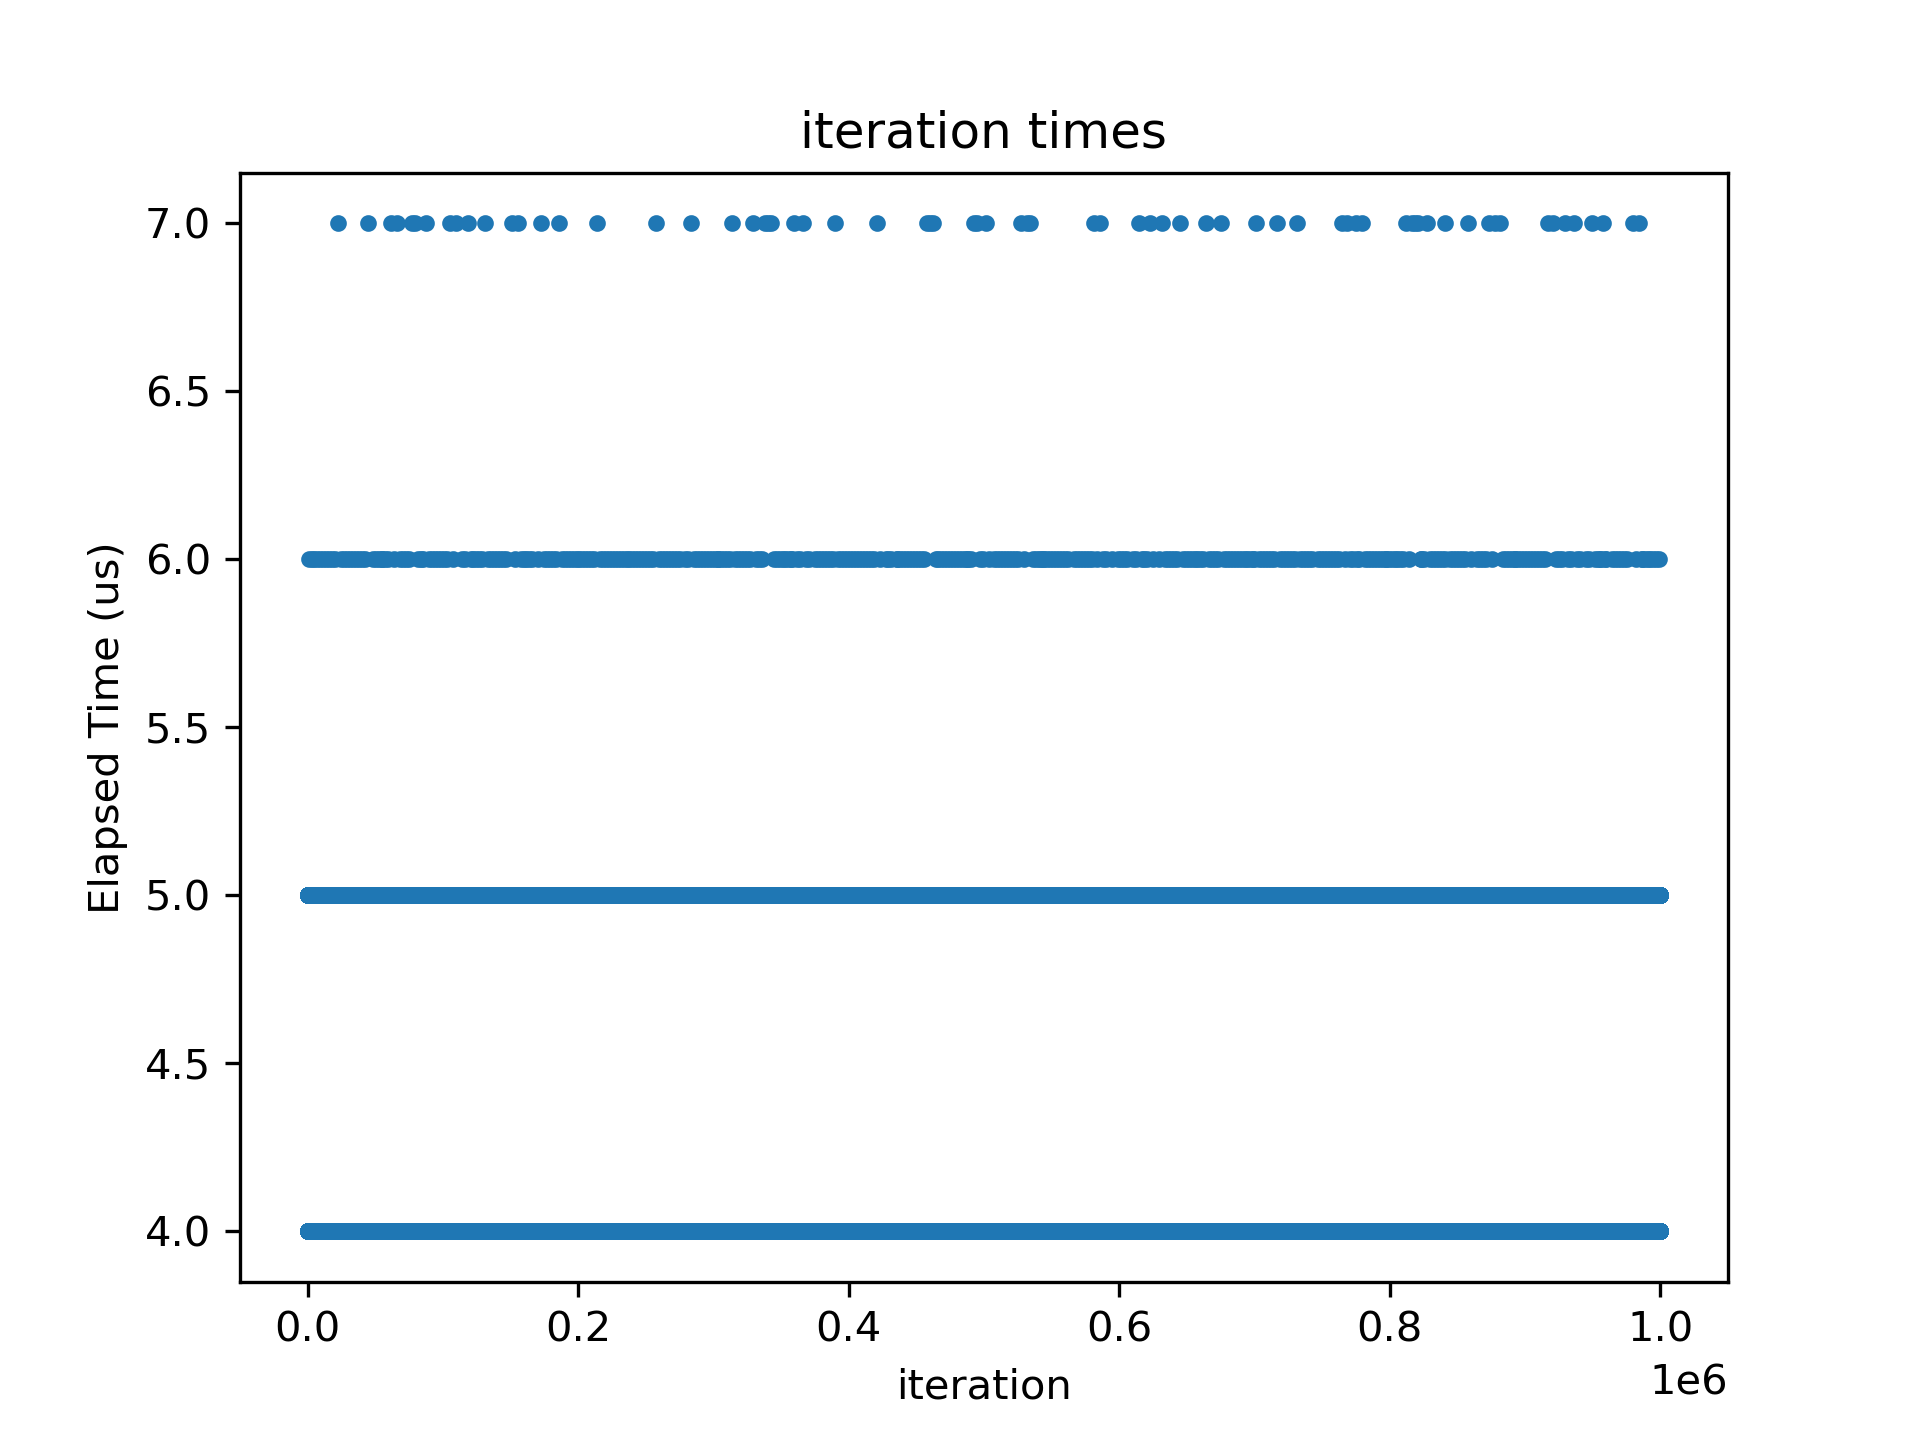
\includegraphics[width=\textwidth]{assets/bare-metal/times.png}
        \caption{The iteration time of every iteration in chronologic order for the bare-metal version}
        \label{fig:experiments:bare-metal:times}
      \end{center}
    \end{minipage}
  \end{center}
\end{figure}

The bare-metal version is the first one we will look at in more detail.
The first observation from the graphs \ref{fig:experiments:bare-metal:hist} and \ref{fig:experiments:bare-metal:times} is that the iteration time values are integer values.
The reason for this is the earlier discussed 1MHz oscillator on the Raspberry Pi, which only allows us to count full microseconds.
With the bare-metal version we are close to the limit of making useful time measurements on the Pi.
The second observation is the consistency of this version.
As can be seen in the histogram, in $99\%$ of the cases the iteration time is four or five microseconds and $99.9\%$ is under seven microseconds.
This is also reflected in the standard deviation of the bare-metal version, which is the lowest of all even when adjusted for the mean.

\begin{figure}[h]
  \begin{center}
    \begin{minipage}{0.48\textwidth}
      \begin{center}
        \includesvggraphics{assets/os-default/hist.svg}
        \caption{Histogram of the iteration times for one million iterations of the linux version without any modifications}
        \label{fig:experiments:os-default:hist}
      \end{center}
    \end{minipage}
    \hspace{0.02\textwidth}
    \begin{minipage}{0.48\textwidth}
      \begin{center}
        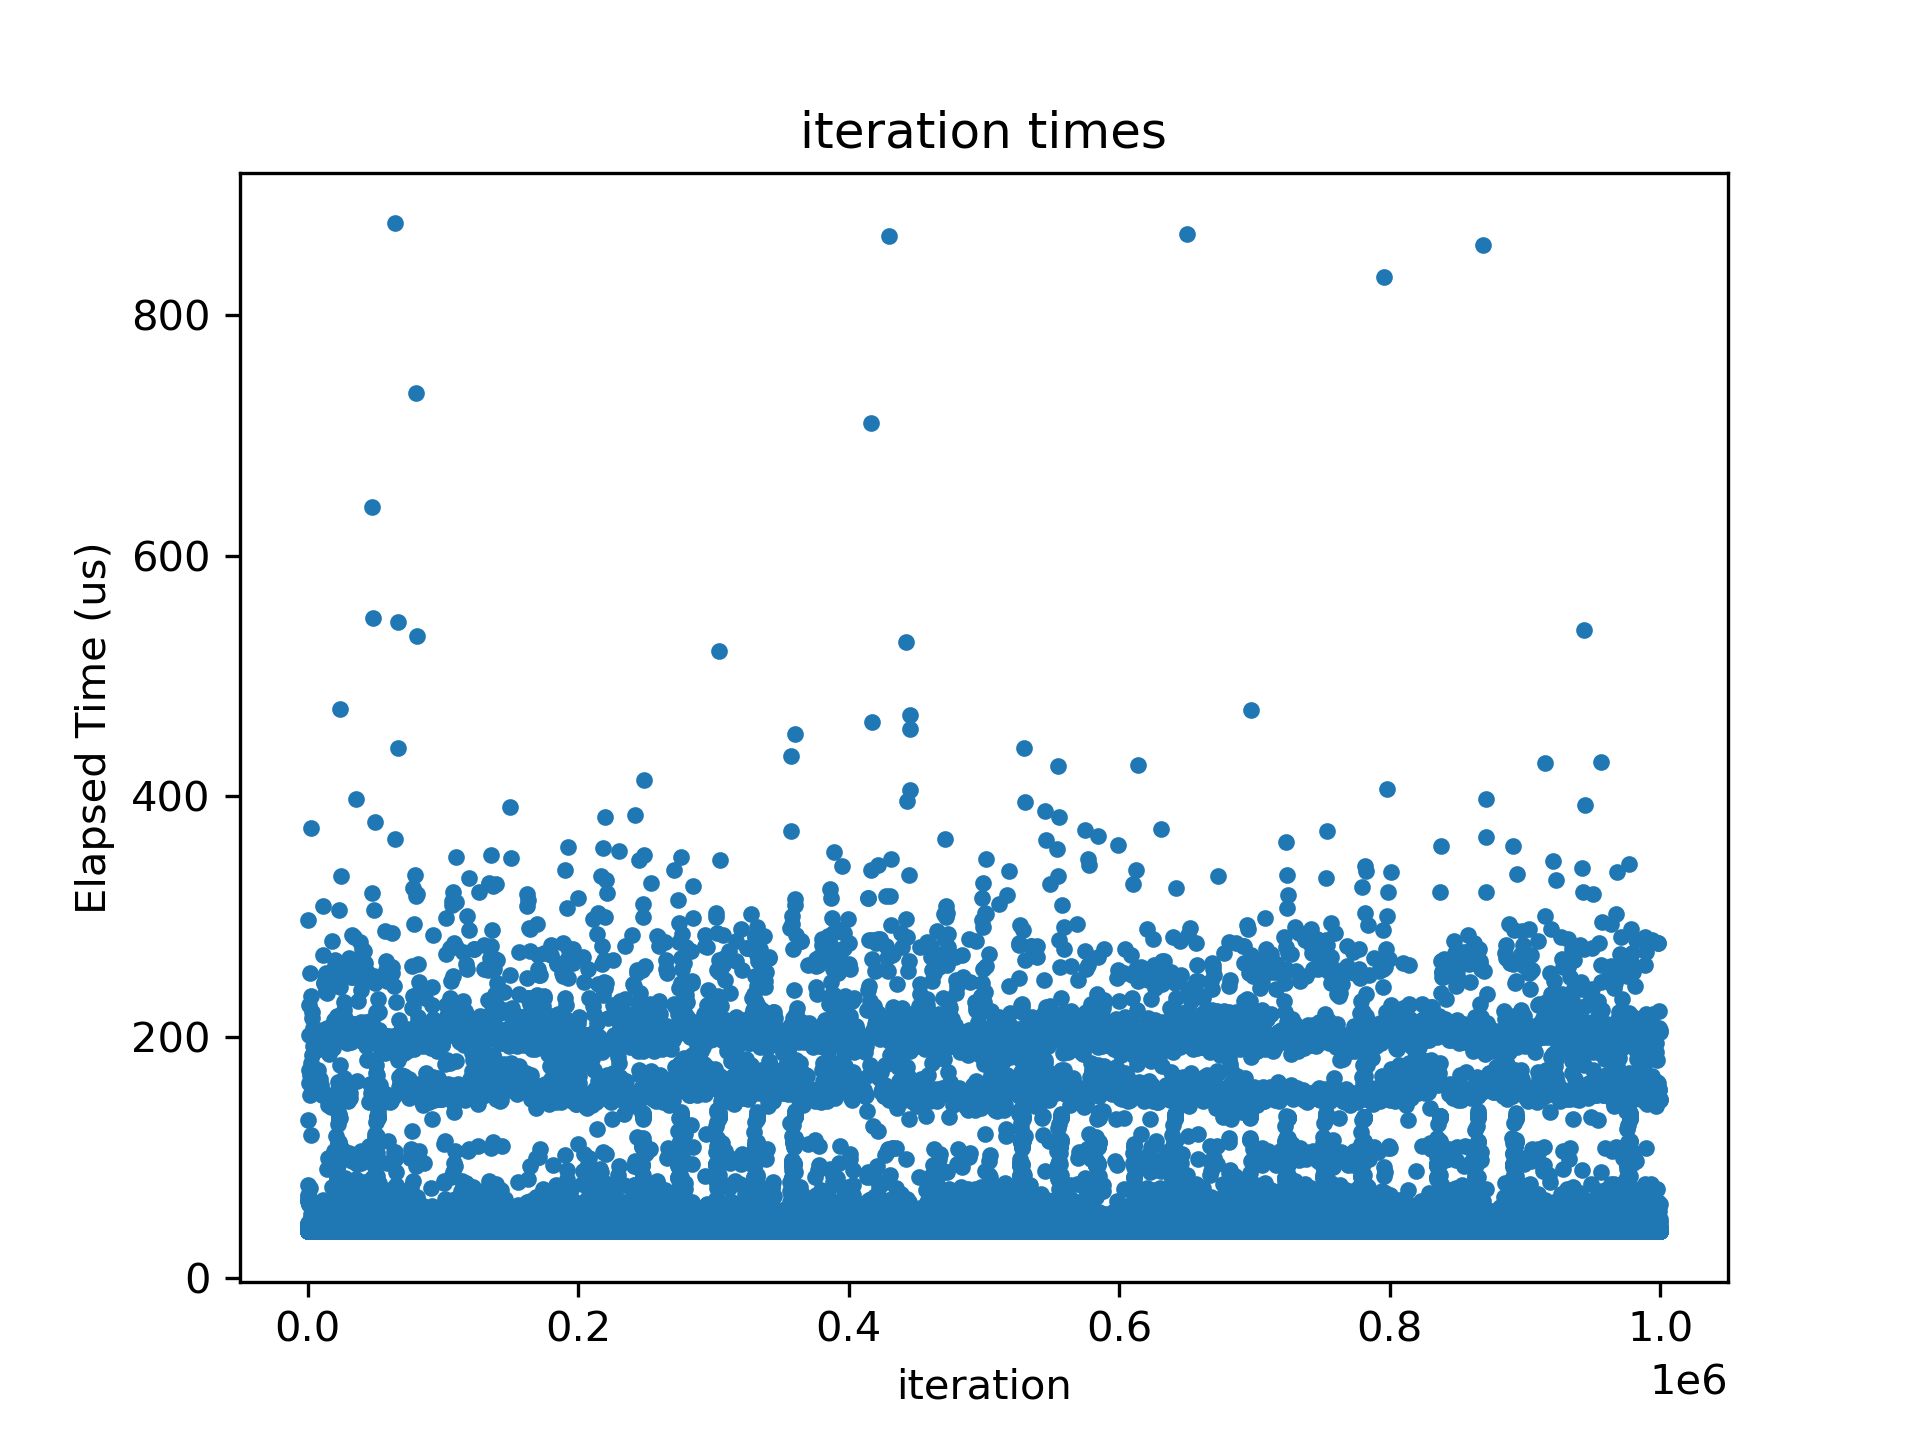
\includegraphics[width=\textwidth]{assets/os-default/times.png}
        \caption{The iteration time of every iteration in chronologic order for the linux version without any modifications}
        \label{fig:experiments:os-default:times}
      \end{center}
    \end{minipage}
  \end{center}
\end{figure}

With the first linux version we also see drastic differences compared to the bare-metal version.
The quantization problem from the bare-metal version is gone, which can be nicely seen in Figure \ref{fig:experiments:os-default:times}, but this is due to the generally higher runtimes.
The average iteration times are about 40.38us, which is about ten times higher than in the bare-metal version, with its 4.4us.
Similar to the bare-metal version, iteration the average iteration times again make up about $99\%$ or the measured times.
The worst-case latencies got disproportionately bigger,
in the bare-metal version they were roughly double the average iteration time with seven vs four microseconds,
here they are over 20 times higher with 876 vs 40 microseconds.
Both higher average and worst-case times we're expected when comparing a bare-metal and linux version,
the disproportionately higher increase in worst-case latencies however is undesireable.

\begin{figure}[h]
  \begin{center}
    \begin{minipage}{0.48\textwidth}
      \begin{center}
        \includesvggraphics{assets/os-isolated/hist.svg}
        \caption{Histogram of the iteration times for one million iterations of the linux version on a reserved core}
        \label{fig:experiments:os-isolated:hist}
      \end{center}
    \end{minipage}
    \hspace{0.02\textwidth}
    \begin{minipage}{0.48\textwidth}
      \begin{center}
        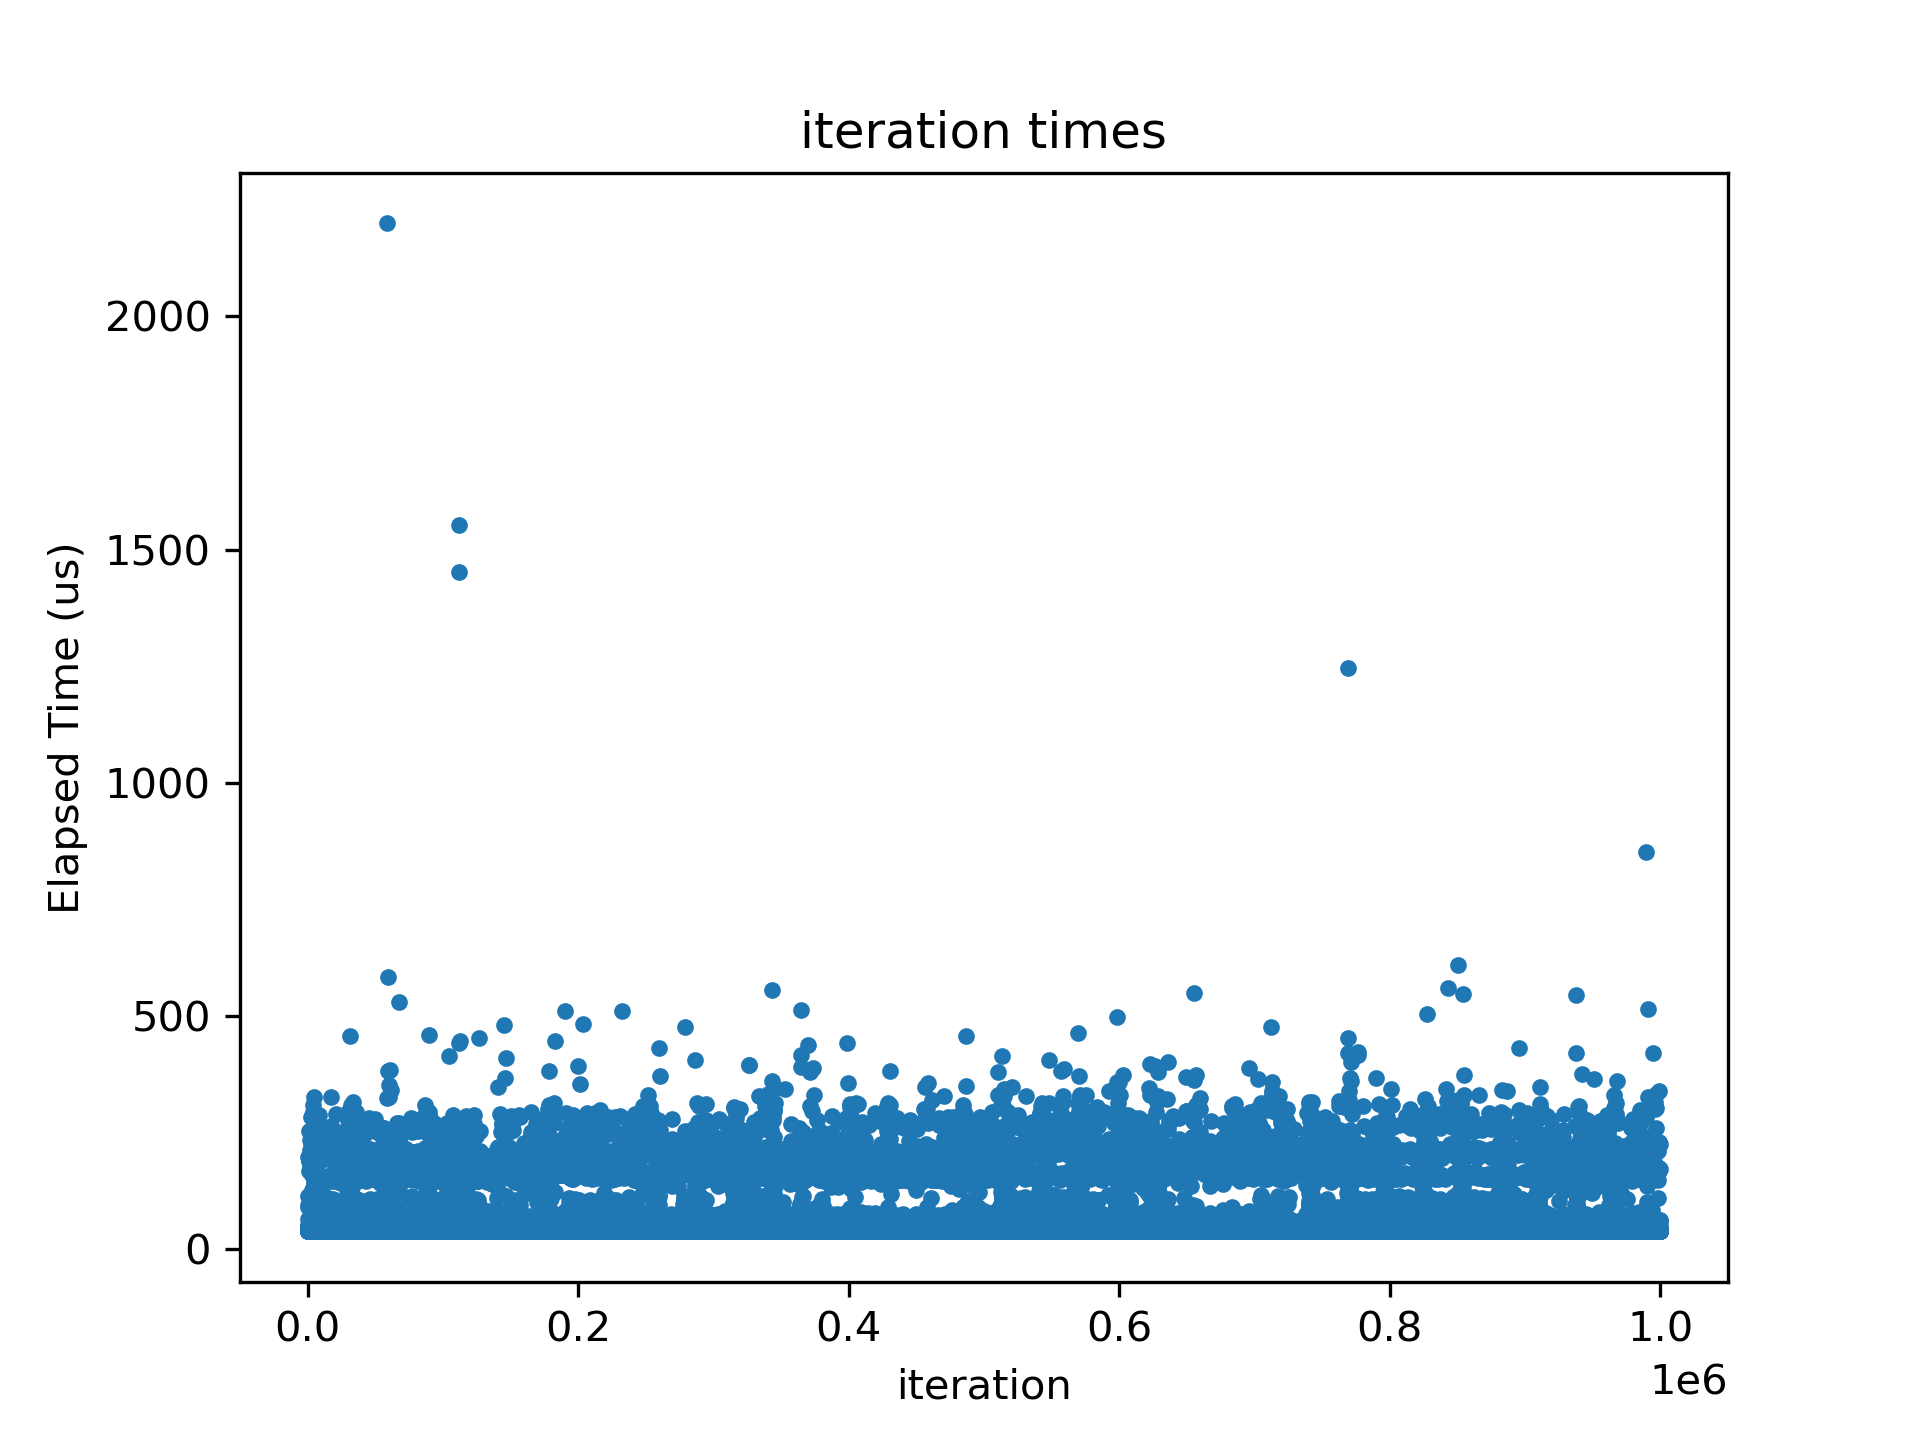
\includegraphics[width=\textwidth]{assets/os-isolated/times.png}
        \caption{The iteration time of every iteration in chronologic order for the linux version on a reserved core}
        \label{fig:experiments:os-isolated:times}
      \end{center}
    \end{minipage}
  \end{center}
\end{figure}

The goal of the isolated core and realtime linux versions was to reduce the expected impact linux had on the worst-case times.
In light of that goal, the most important metric are the worst-case latencies.
When looking at the raw numbers,
the isolated core with 2.2ms and the realtime version with 2.5ms are significantly worse than the standard linux version with its 876us.
There is however an important detail that gets lost in looking only at the worst value.
When comparing the iteration time graphs in figure \ref{fig:experiments:os-default:times}, figure \ref{fig:experiments:os-isolated:times} and figure \ref{fig:experiments:os-rt:times},
we can see that these extreme latencies only occur a handful of times, five times for the isolated core version and two times for the realtime version.
This causes both graphs to be more compressed, hiding the fact that the isolated-core version slightly outperforms the standard linux version.
For the realtime version this does the exact opposite, hiding that even the sub 1ms spikes occur roughly 100 times more often than in both other linux versions.

\begin{figure}[h]
  \begin{center}
    \begin{minipage}{0.48\textwidth}
      \begin{center}
        \includesvggraphics{assets/os-rt/hist.svg}
        \caption{Histogram of the iteration times for one million iterations of the linux version with a realtime kernel}
        \label{fig:experiments:os-rt:hist}
      \end{center}
    \end{minipage}
    \hspace{0.02\textwidth}
    \begin{minipage}{0.48\textwidth}
      \begin{center}
        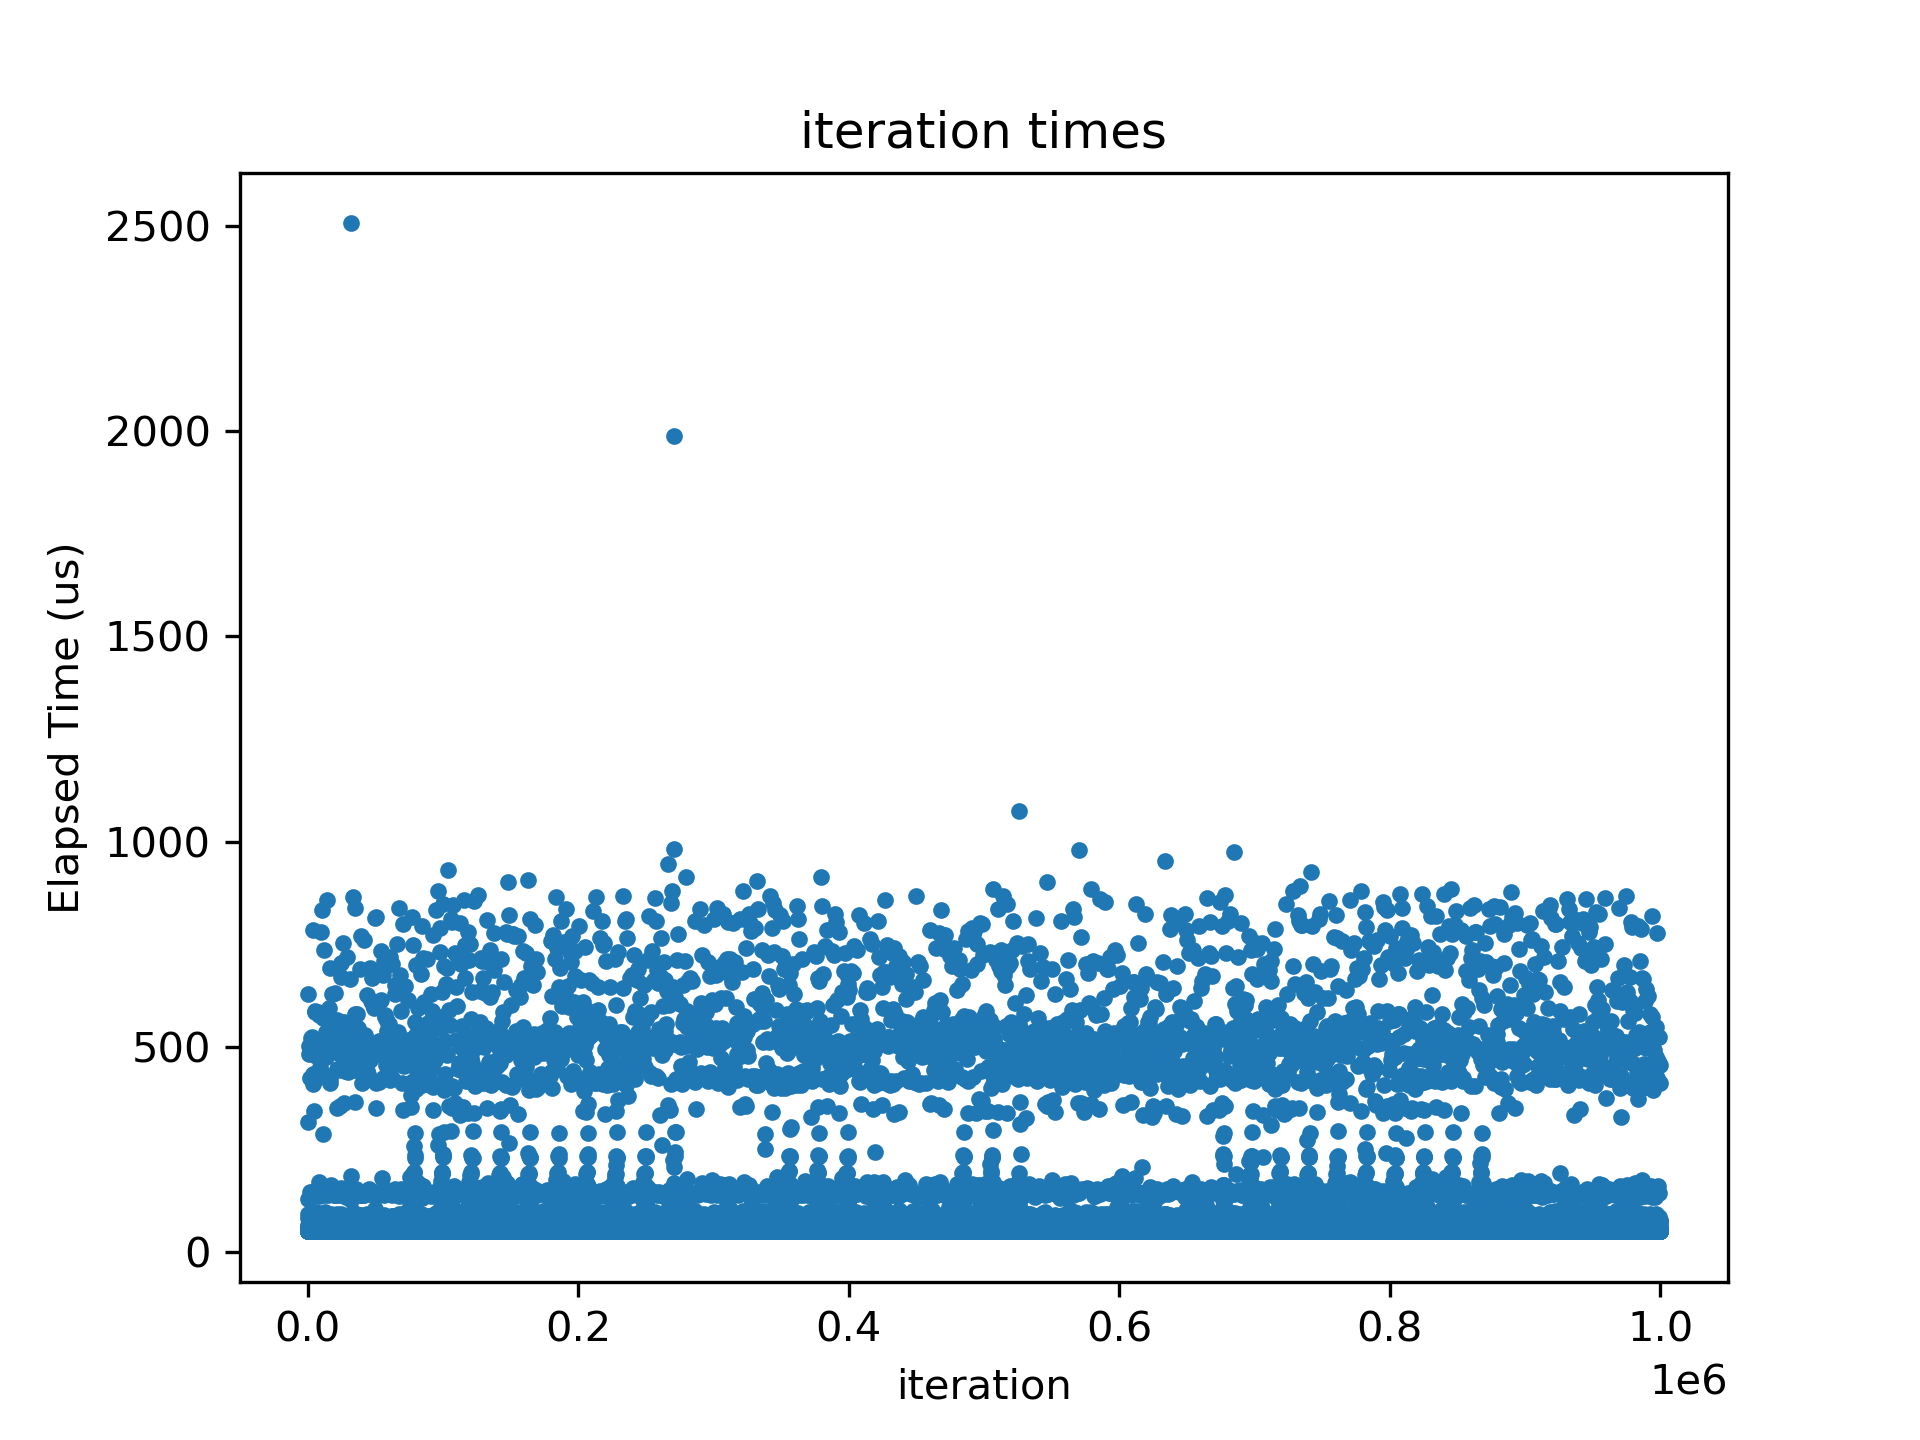
\includegraphics[width=\textwidth]{assets/os-rt/times.png}
        \caption{The iteration time of every iteration in chronologic order for the linux version with a realtime kernel}
        \label{fig:experiments:os-rt:times}
      \end{center}
    \end{minipage}
  \end{center}
\end{figure}

\section{Interpretation}

There are two different things to analyze here.
First, the difference between the bare-metal and linux versions.
All of the linux-based versions have average execution times of an order of magnitude more than the bare-metal version,
which leaves the question:
Is this speed difference adequately explained by the Linux version having to switch the execution context to the kernel and back for the PWM and SPI kernel drivers?
To answer this properly, we profiled a run of the default Linux version, the result can be seen in Figure \ref{fig:experiments:flamegraph}.
From this we can see that most of the time (84.12\%) is spent setting the duty cycle, which in turn means that the context switching overhead is not the issue.
If it were, we would see close to the same duration for SPI and obtain the system time, as we see for PWM.
This can have one of two causes:\\
The Linux kernel PWM driver is very slow.
Or, the rppal implementation of set\_duty\_cycle() is not optimal,
either because it does extra steps not needed for our case,
or talks to the kernel in an inefficient way.
Of these two the second one is more likely for two reasons,
code in the Linux kernel gets significantly more exposure and testing than rppal and the Circle PWM source code states
that it is heavily inspired by the Linux implementation.
If the reason is indeed that rppal could have been programmed differently for this task,
a significant speedup could be achieved.
Assuming the set\_duty\_cycle() was as fast as the SPI transfer,
which would be reasonable since the spi transfer has to write and read to memory and the duty cycle function only has to do one write,
the linux version times would come down to roughly 15us,
putting it in a very comparable ballpark as the bare-metal version.

\begin{figure}[H]
  \begin{center}
    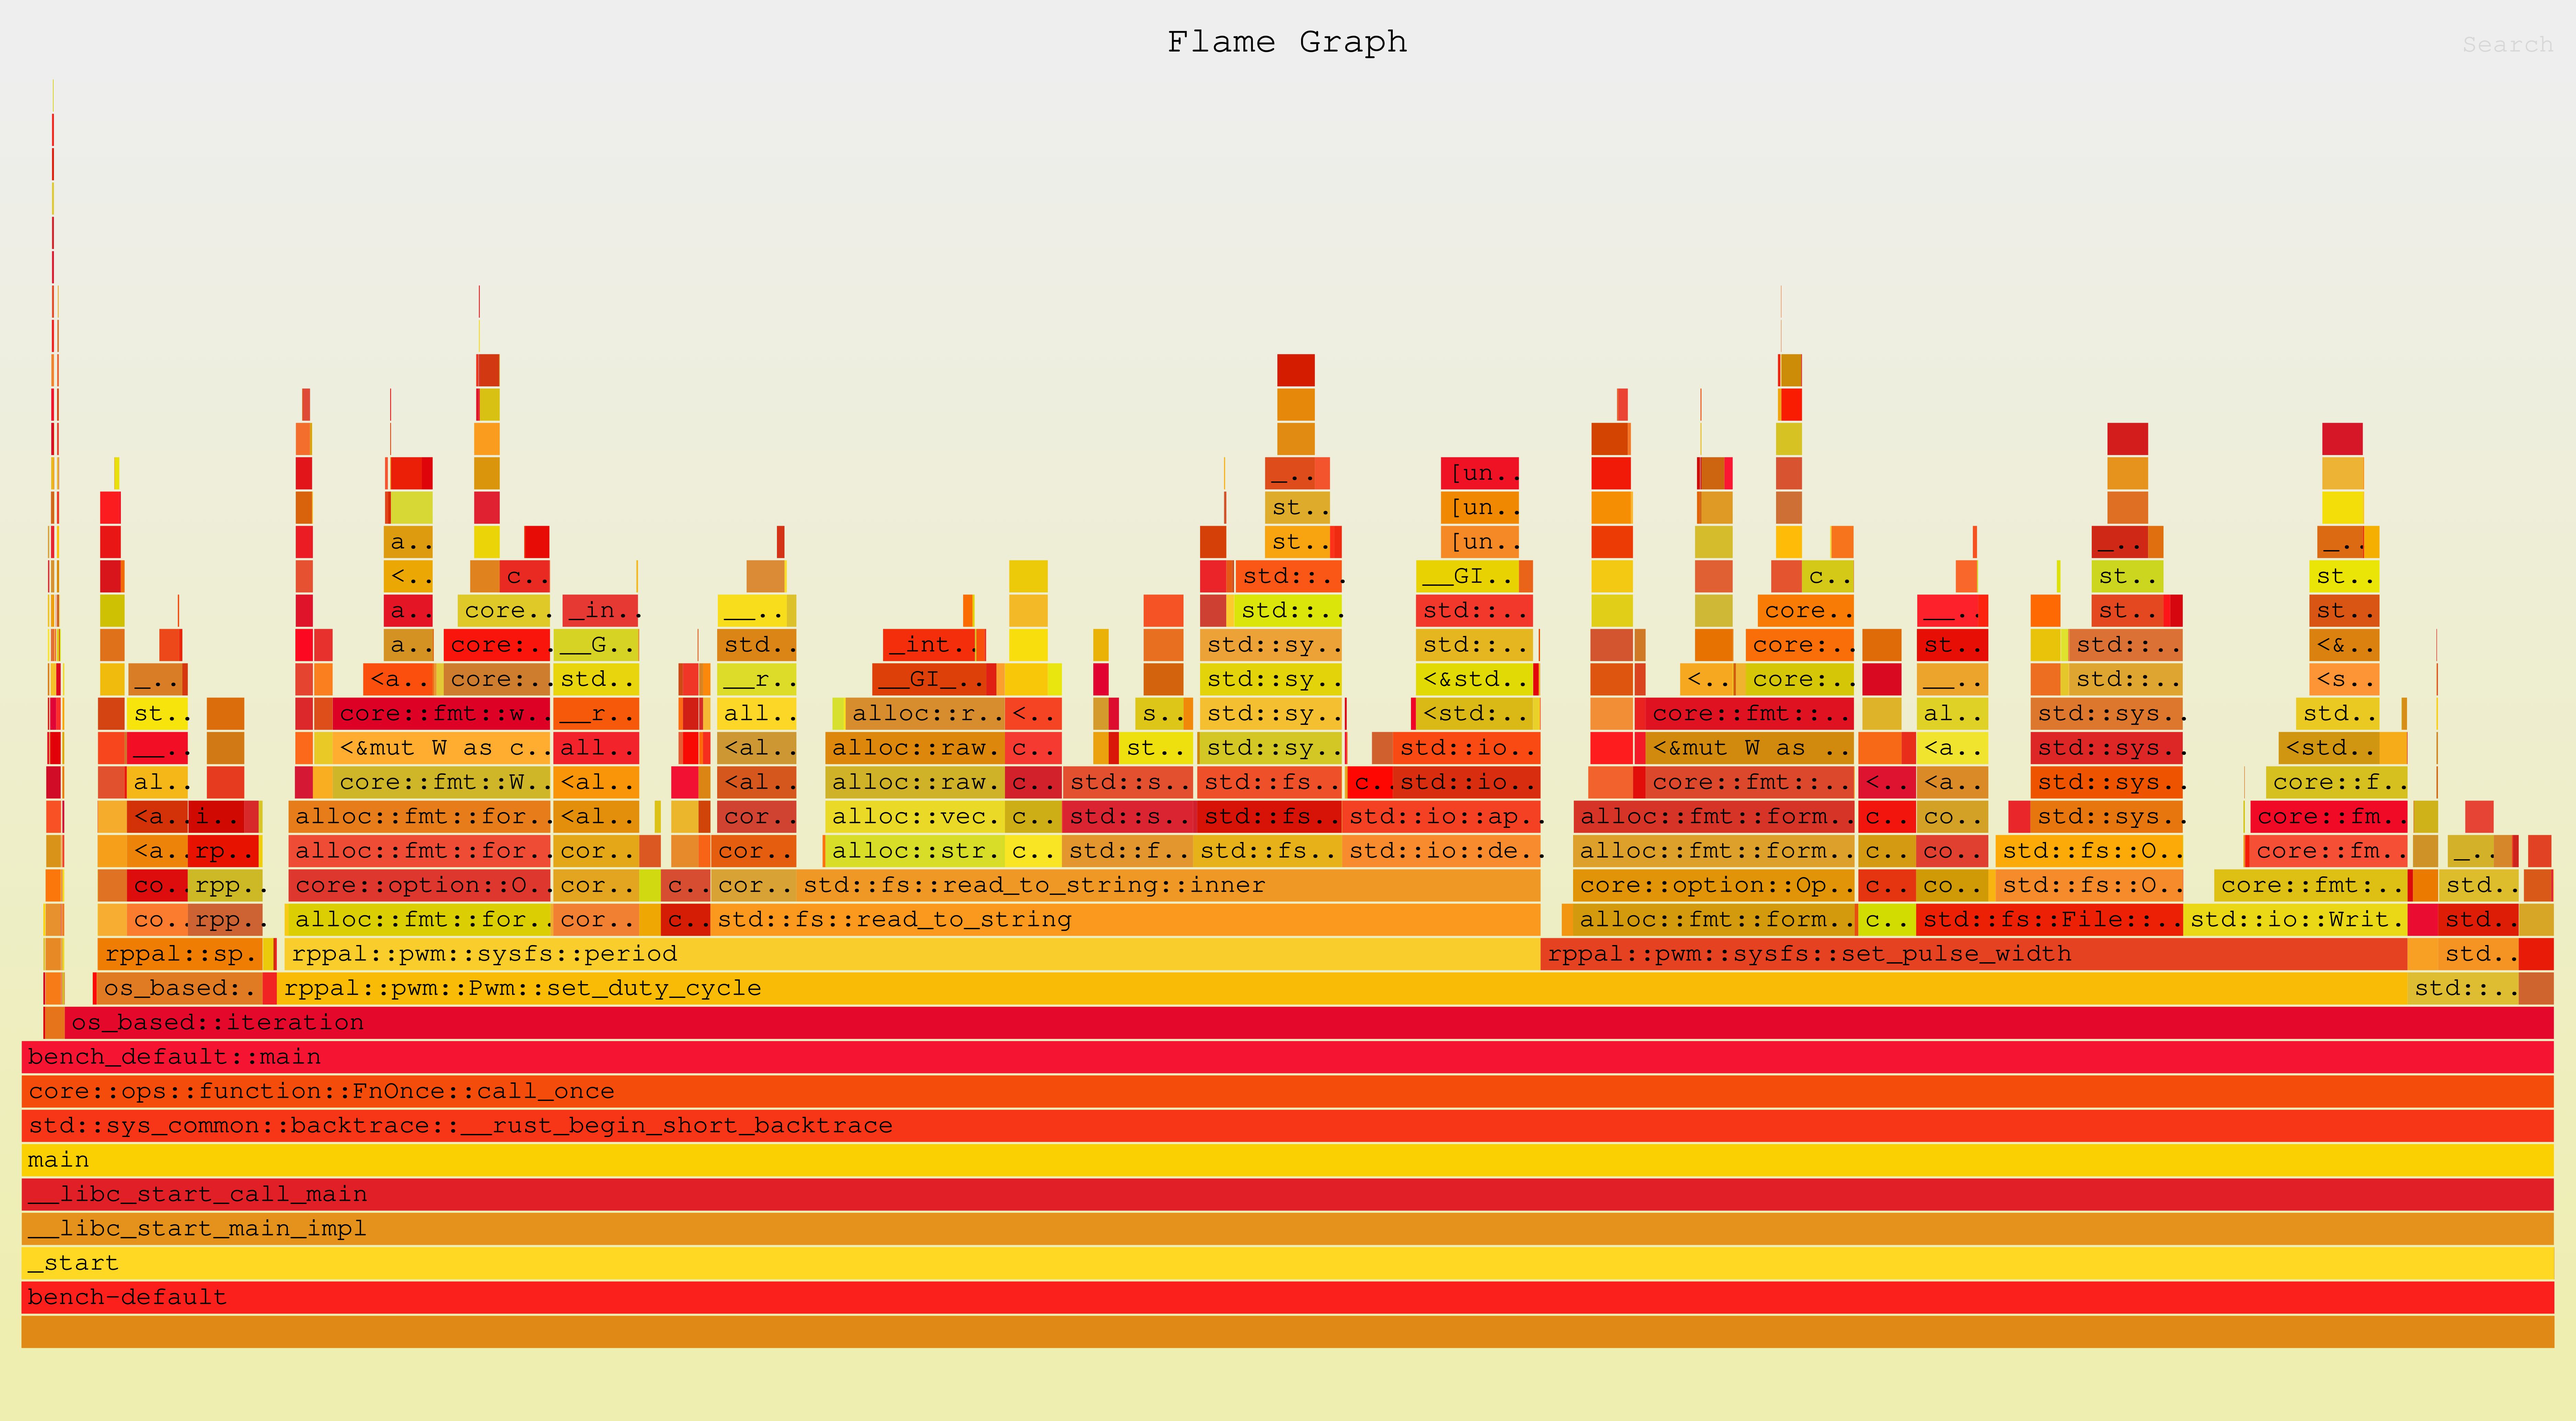
\includegraphics[width=\textwidth]{assets/os-default/flamegraph.png}
    \caption{A flamegraph for the default linux version, with times spent inside of each function}
    \label{fig:experiments:flamegraph}
  \end{center}
\end{figure}

The second part of the results worth analyzing is the comparison of the Linux versions with each other.
The goal of reducing the worst-case latencies on Linux has failed.
Every one of the Linux versions has regular lag spikes to more than an order of magnitude higher than the average iteration time.
The isolated core and real-time versions that we hoped would reduce this behavior show very similar behavior as the stock version for iteration times under 1ms,
but additionally have rare spikes up in the 2-2.5ms region.
These spikes are a major problem, because when implementing a motor controller on top, the possible high reaction times result in several problems:
From a safety perspective, when hitting an obstacle, such as possibly a human, we want the motor to slow down,
but with these spikes the motor could be using its full force on an obstacle for up to 2.5ms.
The second problem is accuracy, in the \nameref{chap:introduction} chapter we discussed that part of the job of a a controller is to prevent large overshoot and oscillation,
both of which become more difficult with higher reaction times.
This is especially important for the intended target application of our motor controller in the CARL \cite[]{CARL} successor,
as balancing a bipedal robot is especially demanding on accuracy.

With both of these results in mind, it is safe to say that the bare metal version is the one more suited for the target application,
as regular reaction time spikes of almost a microsecond are just not acceptable and the lower average iteration times are preferable.


% Here the approach should be discussed related to the initial scope and goal.
% Answer the questions: What did you solve and especially what did you not solve? Give hints for potential extensions as future work.
\chapter{Conclusion}
\label{chap:conclusion}

We initially set out to create a flexible motorcontroller on a RaspberryPi,
with the idea being that different control schemes could easily be implemented in software and tested.
To reach this goal we looked at several different approaches,
both from a detailed look at the implementation as well as the resulting performance characteristics.
For all of the approaches we used the programming language Rust,
whose role in the embedded world is still an area of active research.
While a lot of research focuses on how Rusts powerful static analysis can be applied to embedded systems,
we examined the interaction of Rust with C/C++ libraries.

The different versions we developed were:
\begin{enumerate}
    \item A bare-metal version using the Circle C++ library to access peripherals
    \item A version running on the standard linux kernel using the Rust native rppal library for peripheral access
    \item A variant of the linux version that had one core reserved for it to avoid being interrupted or having to wait for a core to be available.
    \item A second variant of the linux version that exchanges the default linux kernel with one patched with a realtime patchset
\end{enumerate}

When testing these for performance, we found two main results.
For one, the linux based versions all exhibited regular iteration time spikes, of up to 2.5 milliseconds,
while the regular run time was more around 40 microseconds.
In this behavior, the linux based versions did not differ significantly from each other,
so for this workload our approaches at optimizing the thread allocation were unsuccessful.
Second, the bare-metal version performed about 10 times faster than the linux based versions,
all while not having the latency spike problem.

Regarding the usage of Rust we found that most of the added complexity of adding another language is not in the language interaction itself,
but rather in the surrounding tooling such as managing multiple compilers, linkers and build systems to all work together.
This can be seen both as a positive as well as a negative.
The positive side is that the language tools such as bindgen for generating the bindings to the C code are in a good shape both from a usability and stability perspective,
while the negative side is the added build system complexity might deter people that are just trying to code the actual program.

This leaves several directions in which this research could be expanded in future work.
Writing the bare-metal program in C for a performance comparison between Rust with a C++ library and pure C++ would be a logical follow-up to the embedded Rust work.
And on a different route, an in-depth analysis of why and how the latency spikes for the linux version occur could yield results how to achieve comparable performance to the bare-metal version.


\chapter{Appendix}
\label{chap:appendix}

\section{Setting up a Raspberry Pi 4 with a realtime kernel}
\label{sec:appendix:realtime}
This is a short guide on how to reproduce the realtime kernel that we used for all realtime experiments.

To do this you need a Raspberry Pi 4 with a 64Bit Raspberry Pi OS installed (doesn't matter if it's the full desktop version or just a TTY one).

Step 1 is to get all the required build dependencies.
\begin{lstlisting}[language=bash, breaklines]
    sudo apt update && sudo apt install build-essential flex bison libssl-dev bc
\end{lstlisting}

Step 2 is to get the kernel sources and patch them with the correct PREEMPT-RT patchset.
\begin{lstlisting}[language=bash, breaklines]
    wget https://github.com/raspberrypi/linux/archive/refs/tags/stable_20240124.tar.gz
    wget https://cdn.kernel.org/pub/linux/kernel/projects/rt/6.1/older/patch-6.1.73-rt22.patch.xz
    tar -xf stable_20240124.tar.gz
    cd linux-stable_20240124
    xzcat ../patch-6.1.73-rt22.patch.xz | patch -p1
\end{lstlisting}

Step 3 is to generate the kernel config, we use the provided default config for the Raspberry Pi 4 and only set the PREEMPT\_RT config value to enable full kernel preemption.
\begin{lstlisting}[language=bash, breaklines]
    make bcm2711_defconfig
    ./scripts/config -e PREEMPT_RT
    make olddefconfig
\end{lstlisting}

Step 4 is to actually compile the kernel, this takes about 3 hours on all 4 cores of the Raspberry Pi 4.
\begin{lstlisting}[language=bash, breaklines]
    make -j4 Image.gz modules dtbs
\end{lstlisting}

Step 5 is to actually install the files.
\begin{lstlisting}[language=bash, breaklines]
    sudo make modules_install
    sudo cp arch/arm64/boot/dts/broadcom/*.dtb /boot/firmware/
    sudo cp arch/arm64/boot/dts/overlays/*.dtb* /boot/firmware/overlays/
    sudo cp arch/arm64/boot/dts/overlays/README /boot/firmware/overlays/
    sudo cp arch/arm64/boot/Image.gz /boot/firmware/kernel8.img
\end{lstlisting}

At the end simply reboot to load the new kernel.


\RRLABbibliography{literatur}

\RRLABindex

\end{document}
